\documentclass[upright, contnum]{umemoria}
\depto{DEPARTAMENTO DE CIENCIAS DE LA COMPUTACIÓN}
\author{NICOLÁS SALAS VEGA}
\title{DESARROLLO DE UN SISTEMA DE EVALUACIÓN DE POSTULACIONES AL MAGÍSTER EN TECNOLOGÍAS DE LA INFORMACIÓN}
\auspicio{.}
\date{ABRIL 2021}
\guia{SERGIO OCHOA, DANIEL PEROVICH}
\carrera{INGENIERO CIVIL EN COMPUTACIÓN}
\memoria{MEMORIA PARA OPTAR AL TÍTULO DE}
\comision{JUAN ÁLVAREZ, CLAUDIO GUTIÉRREZ}

% Prevenir quiebre de palabras
\tolerance=1
\emergencystretch=\maxdimen
\hyphenpenalty=10000
\hbadness=10000

\usepackage{lipsum}

% \usepackage[latin1]{inputenc}
% \usepackage[T1]{fontenc}

\begin{document}

\frontmatter
\maketitle

\begin{abstract}
    El Programa de Magíster en Tecnologías de la Información (MTI), que imparte
    el Departamento de Ciencias de la Computación de la Universidad de Chile,
    recibe de forma \emph{online} postulaciones de ingreso al programa a través
    de la plataforma UCampus. Estas postulaciones deben ser descargadas por el
    personal de apoyo, y luego evaluadas por miembros del comité académico del
    programa. Estos últimos emiten una recomendación de aceptación o rechazo
    para cada postulación. El coordinador del programa analiza esas
    recomendaciones y emite una resolución al respecto.

    Actualmente, el proceso de evaluación de cada postulación se lleva a cabo a
    través del intercambio de correos electrónicos, coordinados en gran medida
    por el personal de apoyo al programa. Estas personas se encargan de enviar
    los antecedentes a los evaluadores, y solicitar su recomendación de
    aceptación o rechazo, recolectar las recomendaciones, y enviárselas al
    coordinador para que emita una resolución. Todo esto, con las limitaciones
    típicas del intercambio de correos electrónicos en términos de eficiencia
    del procesamiento y la eventual pérdida de información.
    
    Por otra parte, esta forma de procesar las evaluaciones no permite extraer
    estadísticas o mantener la historia de las evaluaciones. Sin datos
    fidedignos acerca del funcionamiento de este proceso, se vuelve difícil
    poder mejorarlo. Hoy en día el MTI representa un canal importante de
    transferencia de conocimiento desde el Departamento hacia la industria, por
    lo tanto, todos sus procesos deben funcionar lo mejor posible.
    
    El objetivo de este trabajo de memoria es desarrollar un sistema que permita
    automatizar gran parte del procesamiento de las postulaciones al MTI,
    alivianando la carga de trabajo sobre las personas involucradas, mejorando
    la gestión de éste, y la capacidad de medir distintos aspectos del proceso.
    
    Para alcanzar el objetivo planteado se desarrolló un sistema web que
    gestiona las evaluaciones de las postulaciones. Éste extrae los datos desde
    UCampus utilizando un scraper, almacena las postulaciones en su base de
    datos, e implementa un workflow que automatiza gran parte del proceso antes
    descrito.
    
    Debido al esfuerzo que requiere la ejecución de dicho workflow, así como el
    número de participantes que intervienen en él, la solución desarrollada fue
    evaluada con postulaciones de prueba (con información ficticia), donde dos
    miembros del comité académico ejecutaron el proceso completo. Durante las
    pruebas, estas personas debieron asumir los distintos roles involucrados en
    el proceso, y tomar las acciones correspondientes a dichos roles.
    
    Como resultado de las pruebas se vió que el sistema soporta correctamente el
    proceso de evaluación de postulaciones, y sólo se indicaron mejoras a la
    usabilidad de las interfaces del mismo. Estas mejoras serán abordadas como
    parte del trabajo a futuro de este proyecto.
    
\end{abstract}

\begin{dedicatoria}
Una dedicatoria corta.
\end{dedicatoria}

\begin{thanks}
\lipsum[1-2]
\end{thanks}

\cleardoublepage
\tableofcontents
\cleardoublepage
\listoftables
\cleardoublepage
\listoffigures

\mainmatter

\begin{intro}
	El Departamento de Ciencias de la Computación de la Universidad de Chile
	ofrece distintos programas de magíster. Uno de ellos es el Magíster en
	Tecnologías de la Información (en adelante MTI). Uno de los objetivos de
	este programa es formar especialistas con conocimientos de aspectos
	aplicados respecto al uso, gestión y adopción de Tecnologías de la
	Información y Comunicaciones.

	Teniendo en cuenta el perfil de los profesionales que busca formar este
	programa, y la naturaleza misma del magíster, resulta razonable pensar que
	el proceso de postulación al mismo, así como el procesamiento de dichas
	postulaciones, se haga usando herramientas computacionales.
	
	Hoy en día, la postulación a este programa se hace a través de la plataforma
	UCampus\footnote{UCampus es un Centro Tecnológico que desarrolla plataformas
	de apoyo a la gestión, automatizando los procesos de Instituciones de
	Educación Superior, en particular el de la Universidad de Chile.
	https://ucampus.cl.}. En esa plataforma, el postulante debe ingresar sus
	datos personales, y adjuntar un conjunto de documentos relevantes para
	respaldar su  postulación. Entre esos documentos están las cartas de
	recomendación, el currículum del postulante, su certificado de título y su
	carta motivacional.
	
	Una vez enviada la postulación a través de UCampus, los documentos quedan
	disponibles para que cada programa (en este caso, el MTI) haga con ellos lo
	que estime conveniente. UCampus no ofrece la funcionalidad para apoyar el
	procesamiento de las postulaciones, por lo que cada programa debe hacerlo
	por fuera de esta plataforma. 

	\section{Problema Abordado}

	El proceso de evaluación de postulaciones al MTI se realiza en forma manual.
	Para ello, un funcionario del Programa de Educación Continua (PEC) del DCC
	inicia el proceso descargando manualmente cada uno de los archivos subidos a
	UCampus por el postulante. Esa información luego es enviada a los miembros
	del comité académico del programa a través de un correo electrónico. Los
	miembros de ese comité evalúan las postulaciones. Estas personas pueden
	solicitar información adicional al postulante en caso que se requiera; y en
	esos casos, el funcionario del PEC actúa como intermediario entre el
	postulante y el comité académico.

	Cuando la información de una postulación está completa, los evaluadores emiten
	un juicio individual y justificado respecto a la admisión o no de cada
	postulante al programa. Esta información es enviada vía correo electrónico al
	funcionario del PEC, quien reúne todas las opiniones de los evaluadores acerca
	de una postulación, y luego se las envía al coordinador del programa para que
	decida la admisión o rechazo del postulante. En esa instancia, el coordinador
	revisa manualmente todas las evaluaciones y emite un juicio formal, el cual debe
	ser registrado en la plataforma UCampus, e informado al postulante.

	Este flujo de trabajo (workflow) es completamente informal, por lo que los
	tiempos de procesamiento de una postulación varían mucho, dependiendo de la
	carga de trabajo que tengan los funcionarios del PEC y el resto de los
	participantes. Dado que hoy en día las evaluaciones de las postulaciones se
	realizan de forma manual, el proceso se vuelve lento, costoso y propenso a
	errores. Además, el flujo de trabajo asociado a este proceso es muy difícil de
	monitorear, medir y mejorar. Otro aspecto importante es que este proceso manual
	no escala bien, por lo que se requieren sistemas de apoyo al procesamiento de
	estas postulaciones.

	Tomando en cuenta lo anterior, en esta memoria se diseñó e implementó un sistema Web que:

	\begin{enumerate}
		\item Agiliza el proceso de evaluación de postulaciones al MTI.
		\item Facilita la recopilación y almacenamiento de datos relevantes,
		tanto del postulante como de la evaluación de su postulación.
	\end{enumerate}

	El sistema no busca extender la funcionalidad de UCampus, ni la validez de
	la postulación, por lo tanto, en la memoria se asume que los datos que
	provienen de dicha plataforma son correctos. 

	\section{Objetivos de la Memoria}

	El objetivo general de esta memoria fue desarrollar un sistema Web que
	automatiza parte del flujo de trabajo asociado al procesamiento de
	postulaciones al Magíster en Tecnologías de la Información; programa que es
	impartido por la Escuela de Postgrado de la FCFM\footnote{Facultad de
	Ciencias Físicas y Matemáticas de la Universidad de Chile} a través del
	DCC\footnote{Departamento de Ciencias de la Computación}. Los objetivos
	específicos definidos para alcanzar el objetivo general fueron los
	siguientes:

	\begin{enumerate}
		\item Desarrollar un servicio de software que extraiga automáticamente
		la información de las postulaciones al programa, desde la plataforma
		UCampus.
		\item Desarrollar un sistema que automatice el flujo de trabajo
		(workflow) de evaluación de las postulaciones.
		\item Desarrollar un servicio que facilite la toma de decisiones del
		Coordinador del Programa, respecto a la aceptación o rechazo de los
		postulantes, y a la comunicación de éste con la Escuela de Postgrado.
	\end{enumerate}


	\section{Estructura del Documento}
	**Falta añadir aquí la estructura del documento**.
\end{intro}
\chapter{Análisis del escenario legado}

A continuación se indican los roles de los participantes en el proceso de
evaluación de postulaciones. Luego se describe y discute dicho proceso.
Finalmente, se analizan las alternativas para extraer la información de las
postulaciones desde UCampus, y de esa manera poder alimentar el sistema
desarrollado en esta memoria.

\section{Participantes en el Proceso de Evaluación de Postulaciones}

% Wrappear la tabla...
\begin{table}[ht]
    \begin{center}
        \begin{tabular}{|l|l|}
            \hline \\
            Rol & Descripción \\ \hline

            Postulante & Genera una postulación a través de UCampus. Una vez
            entregada la postulación completa, éste espera por el resultado
            (aceptación o rechazo) de la misma.\\ \hline

            Miembro del Comité Académico del Programa & Evalúa las
            postulaciones, emite un voto y entrega su opinión al Coordinador de
            Magíster en forma de comentarios. Estos comentarios justifican la
            opinión del miembro correspondiente respecto a la aceptación o
            rechazo de un postulante \\ \hline

            Coordinador de Magíster / Presidente del Comité Académico & Resuelve
            una postulación. La decisión es tomada en base a las evaluaciones
            realizadas por los miembros del comité. \\ \hline

            Asistente / Funcionario del PEC & Se encarga de revisar la validez
            de los documentos adjuntados a la postulación, y deriva la
            información al Coordinador del Magíster y a los miembros del Comité
            Académico del Programa cuando corresponde. Los asistentes
            (funcionarios) son quienes llevan a cabo la mayor parte del workflow
            manual involucrado en el procesamiento de las postulaciones. \\ \hline
        \end{tabular}
    \end{center}
\end{table}


\section{Proceso a apoyar}

Tomando en cuenta el rol de cada actor, a continuación se resume el proceso que
sigue una postulación hasta lograr un veredicto de aceptación o rechazo.

% Figura
\begin{figure}[!ht]
    \begin{center}
        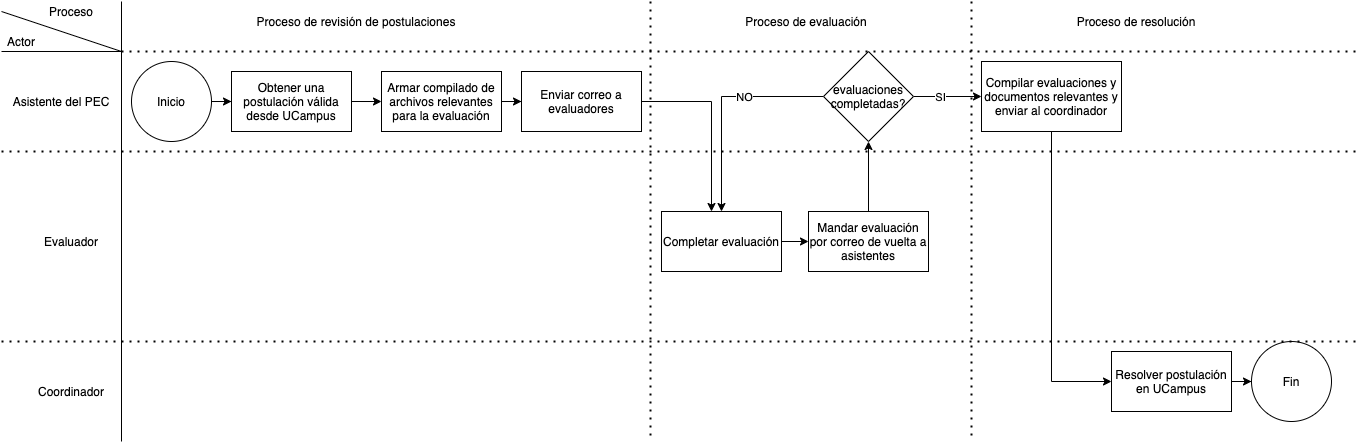
\includegraphics[scale=0.3]{imagenes/01-workflow-legado.png}
    \end{center}
    \caption{Workflow del proceso de evaluación de postulaciones}
    \label{workflow-legado}
\end{figure}

Tal como se puede ver en la figura \ref{workflow-legado}, el proceso involucra
los siguientes 7 pasos:

\begin{enumerate}
    \item Un postulante ingresa una postulación a través de UCampus.
    \item Los asistentes revisan la validez y completitud de la postulación. En
    caso de ser válida y estar completa, la información asociada a ésta se envía
    al Coordinador del Programa y a los Miembros del Comité Académico vía correo
    electrónico.
    \item El Coordinador del Programa y los Miembros del Comité Académico
    evalúan cada postulación, y emiten un juicio individual acerca de la
    aceptación o rechazo del postulante al programa, teniendo en cuenta las
    exigencias establecidas en la normativa vigente del MTI.
    \item Cada evaluador envía por correo sus evaluaciones al asistente, quien
    las recolecta y envía al Coordinador del Programa el conjunto de todas las
    evaluaciones recibidas.
    \item El Coordinador del Programa revisa todas las opiniones de los
    evaluadores y emite un veredicto acerca de la aceptación o rechazo del
    postulante.
    \item El Coordinador del Programa registra la decisión en UCampus y entrega
    a los asistentes un formulario de resolución firmado.
    \item Los asistentes envían el formulario a la Escuela de Postgrado, quien
    notifica al postulante.
\end{enumerate}

En el paso 2, la postulación puede ser devuelta al postulante para que corrija
errores en caso de que existan, o para que éste envíe los documentos faltantes.
Después de una revisión del proceso con el coordinador del programa y miembros
del comité académico, se determinó que el diseño del mismo era apropiado. Las
falencias del mismo radican principalmente en la artesanalidad e informalidad
con la que se realizan las actividades que son parte del mismo. Por lo tanto, la
automatización de algunas de esas actividades parece ser suficiente para mejorar
considerablemente la calidad y predictibilidad del proceso en términos de su
duración.

\section{Obtención de Datos desde la Plataforma UCampus}

Respecto de la obtención de datos de las postulaciones (desde UCampus), a pesar
de que exista una API publicada por su equipo desarrollador, ésta no incluye
end-points que permiten obtener los datos de las postulaciones al magíster, lo
cual va en contra del primer propósito: “permitir agilizar el proceso de
postulaciones”. 

Para resolver este problema, una solución que no involucra trabajo extra de los
usuarios es hacer \emph{scraping} de la página de postulaciones de UCampus. En
ella se muestra una tabla con todas las postulaciones y un link de detalle a
cada una de ellas, desde donde se puede obtener la información de todas las
postulaciones al programa. Teniendo esta información, ya sea vía scraping o via
una extensión a la API de UCampus, es posible construir un proceso autónomo que
recupere la información de las postulaciones, sin que se requiera coordinación
manual del proceso por parte de los Asistentes o del Coordinador del Programa.

Para agilizar el procesamiento de las postulaciones, el sistema enviará avisos a
los usuarios relevantes cuando se requiere que tomen alguna acción, evitando así
que estos tengan que estar pendientes de ingresar al sistema para ver si tienen
alguna asignación sobre la cual responder. Un estudio realizado por la empresa
Microsoft constató que este envío de avisos concientiza a las personas de que
hay cosas pendientes, y aunque distrae, es preferido por su valor en la
concientización [1].

Con respecto a la facilidad de recopilación y almacenamiento de los datos
relevantes de los postulantes, usar una base de datos para dicho propósito es
mejor que mantener los datos en las cuentas de correo de los participantes en el
proceso. Si bien algunos datos están disponibles en UCampus (como los resultados
de las postulaciones, por ejemplo), las opiniones de los Miembros del Comité
Académico, entre otros datos, quedan en la cadena de correos asociada a una
publicación. Usando una base de datos, estos datos serán luego fáciles de
acceder, por ejemplo, para realizar un análisis de la efectividad y eficiencia
del procesamiento de las postulaciones.

El desarrollo de este sistema cuenta con los siguientes desafíos:

\begin{enumerate}
    \item UCampus no entrega información estructurada respecto a postulaciones
    al magíster, y se pretende que la alimentación de datos sea realizada de
    forma automática.
    \item El sistema debe automatizar el flujo de trabajo, invitando a los
    participantes (roles involucrados en el proceso) a completar sus tareas lo
    más rápido posible, manteniéndolos informados acerca de tareas que
    eventualmente ellos tengan pendientes de realizar.
    \item El sistema debe garantizar que cada actor del proceso pueda hacer sólo
    lo que su rol permite, y nada más.
\end{enumerate}


\section{Análisis de Alternativas de Interacción con UCampus}

En esta sección se describen las tareas realizadas en la búsqueda de una
solución a la extracción automática de información desde UCampus. En particular
se indican los desafíos asociados a los problemas que hay que resolver, las
alternativas para abordarlos y las propuestas de solución.

\subsection{Posible Extensión de la API de UCampus}

Una de las primeras tareas realizadas fue comunicarse con el área de desarrollo
de UCampus, para explorar la factibilidad de implementar un nuevo endpoint en su
API, con el objetivo de permitir la extracción de los datos de las postulaciones
desde una aplicación externa; en este caso, nuestro sistema de evaluación. Si
bien la respuesta fue pronta y con buena disposición, no se dió curso a la
solicitud por las siguientes razones:

\begin{itemize}
    \item El formulario de ingreso de datos y el flujo de una postulación están en
    el sistema llamado ``Workflow'', el cual está a cargo del ADI (Área de
    Infotecnologías), y por lo tanto, poco puede ayudar el Centro UCampus a la
    intervención de dicho sistema. Además, no hay una conexión directa entre el
    sistema de ADI y la plataforma UCampus, por lo que se requiere realizar bastante
    trabajo para poder contar con información de postulaciones a través de la API de
    UCampus.
    \item La respuesta desde ADI fue que los datos se encuentran encapsulados dentro
    de herramientas internas del sistema ``Workflow'', lo cual dificulta la extracción
    de datos limpios desde su base de datos.
\end{itemize}

En resumen, y aunque aún no está completamente cerrada la posibilidad de obtener
los datos desde la fuente, se hace necesario explorar otras opciones, las cuales
se detallan a continuación.

\subsection{Extracción de Datos de UCampus Usando Scrapers}

Scraping es una técnica que se usa para la extracción de datos no estructurados,
ya sea a partir de imágenes, PDFs, o páginas web, entre otros. Al no poder
obtener directamente los datos de postulaciones a través de una API (o una
interfaz de acceso a datos similar), usar un scraper es una buena alternativa
para recuperar dicha información. En este caso, los datos de las postulaciones
se encuentran accesibles a través de una interfaz Web de la plataforma UCampus,
siempre que se cuente con los derechos para ello. Este es el canal oficial tanto
para postular, como para gestionar las postulaciones.

El uso de scrapers no está exento de desafíos. Algunos de los más conocidos son
los siguientes: 

\begin{itemize}
    \item Si el sitio web que representa la fuente de datos cambia su interfaz
    de usuario, entonces se debe adaptar el scraper para extraer información del
    nuevo layout de la página.
    \item Algunos sitios web (y este es el caso de UCampus) usan Javascript en
    su interfaz (versiones modernas). Esto hace que no sea trivial la extracción
    de los datos, pues el scraper debe esperar por eventos asíncronos para poder
    extraer datos. Las librerías tradicionales de scraping [6, 7] no cuentan con
    esa capacidad.
\end{itemize}

A pesar de lo planteado anteriormente, usar un scraper es realmente la única
alternativa que existe hoy para poder extraer los datos de las postulaciones de
forma automática. Con respecto a las alternativas para hacer el scraping, se
analizaron las siguientes librerías, dado que están dentro de las más
reconocidas:

\begin{itemize}
    \item \emph{Puppeteer} [3]: Librería Node.js que permite controlar una instancia de
    Chrome a través del protocolo DevTools.
    \item \emph{Selenium WebDriver} [4]: Esta es una API con implementación en
    múltiples lenguajes, orientada al testing, que permite manejar un browser.
\end{itemize}

Las diferencias entre estas librerías radica principalmente en que Puppeteer
controla instancias de Chrome, mientras que Selenium es una implementación para
un navegador genérico. Ambas cumplen el propósito de extraer datos desde UCampus
sin problemas [8]. En el repositorio referenciado se muestran los resultados de
extraer ciertos datos desde UCampus con la cuenta del autor, de acuerdo a la
siguiente secuencia de pasos:

\begin{enumerate}
    \item Ingresar a UCampus con usuario y contraseña.
    \item Hacer clic en la pestaña Tareas Iniciadas.
    \item Extraer links desde una tabla. Cada caso particular (postulación)
    corresponde a una “Solicitud de Inscripción con Excepción (SIEs)”.
    \item Visitar todos los links disponibles y extraer sus datos.
\end{enumerate}

Con el objetivo de mantener la estabilidad del scraper, en el sentido de que
éste soporte la mayor cantidad de alternativas posibles para abordar los
eventuales cambios en la interfaz de usuario, puppeteer es la mejor opción. El
hecho de que la librería esté construida sobre Chromium hace que se pueda usar
todo el abanico de herramientas de Chrome para obtener datos, y manipular el
sitio web. Otro argumento para lo mismo es la frecuencia de actualizaciones. Los
drivers de Selenium mantienen su última fecha de liberación (para Python) el 1
de noviembre de 2018, mientras que Puppeteer lanzó su última versión el 26 de
febrero de 2021.

Debido a esto, y tomando en cuenta la cantidad de postulantes al MTI, resulta
válido también explorar la posibilidad de que los datos sean ingresados
manualmente al sistema por parte de sus usuarios; particularmente, por los
funcionarios del PEC.

\subsection{Carga Manual de datos de Postulaciones}

Si bien lo ideal es que los datos sean ingresados de forma automática al
sistema, no hay que perder de vista que el objetivo principal de este trabajo
es: \emph{desarrollar un sistema Web que automatice el flujo de trabajo asociado
al procesamiento de postulaciones al Magíster en Tecnologías de la Información}.
Con eso en cuenta, la carga manual de datos se percibe más bien como un
despropósito en este escenario.

Por otra parte, los scrapers anteriormente descritos fueron probados con
resultados satisfactorios que, en una primera aproximación, demostraron que es
posible extraer datos no estructurados desde UCampus, y confiar en los
resultados de dicho proceso. 

\section{Formulario de Postulación al MTI}

A continuación se muestra un formulario típico de postulación al MTI,
implementado sobre la plataforma UCampus. Se han ofuscado los datos sensibles
del postulante.

\begin{figure}[!ht]
    \begin{center}
        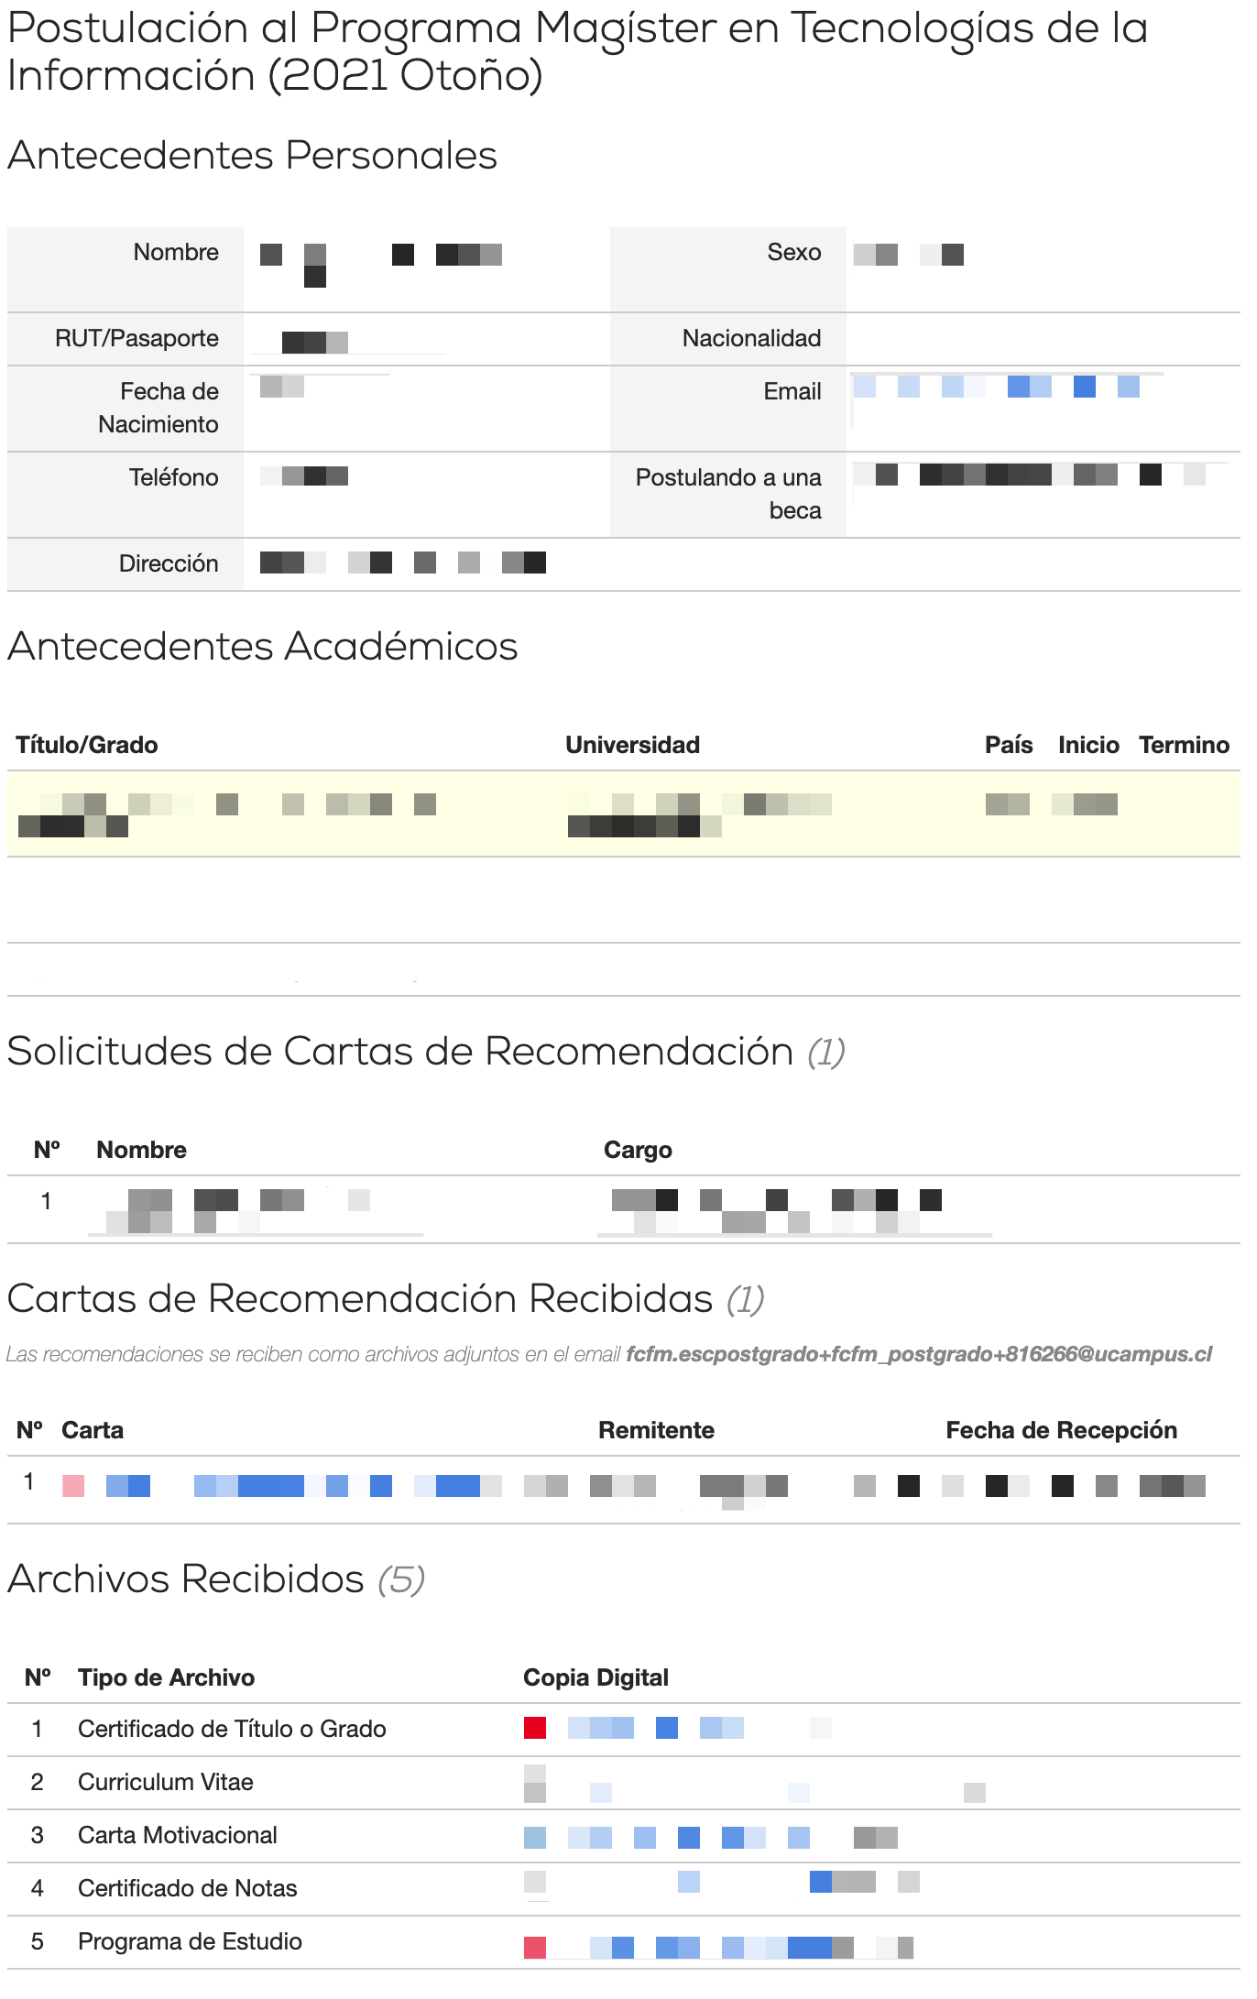
\includegraphics[scale=0.3]{imagenes/01-formulario-postulacion.png}
    \end{center}
    \caption{Formulario de postulación al Magíster en TI}
    \label{formulario-postulacion}
\end{figure}

Como se puede ver en la Figura \ref{formulario-postulacion}, una postulación
completa consta de los siguientes antecedentes:

\begin{itemize}
    \item Datos personales del alumno.
    \item Los antecedentes académicos del mismo: Título o grado, Universidad, País
    de la Universidad, Año de inicio y término de sus estudios.
    \item Solicitudes de cartas de recomendación, hechas por el postulante. Éstas se
    muestran por el nombre de cada persona a la que se le solicitó una carta de
    recomendación, su correo electrónico y su cargo.
    \item Cartas de recomendación recibidas. Éstas muestran el archivo
    correspondiente a la carta de recomendación, el nombre de la persona que lo
    envió, su email y la fecha de recepción.
    \item Los 5 archivos mandatorios de cada postulación: Certificado de título o
    grado, currículum vitae, carta motivacional, certificado de notas y el programa
    de estudio.
\end{itemize}

Algunas consideraciones a destacar del formato de los datos:

\begin{itemize}
    \item La fecha de nacimiento de un alumno sólo está presente para usuarios
    antiguos de UCampus. Usualmente ese campo sólo muestra la edad.
    \item La nacionalidad, de la misma forma, no suele estar presente en la
    postulación.
    \item La postulación puede estar a medio hacer. Vale decir, puede ser que la
    postulación no contenga las cartas de recomendación o documentos esenciales,
    y aún así el sistema permite que la misma sea enviada al coordinador del
    programa.
\end{itemize}
\chapter{Concepción de la Solución}

En este capítulo se presenta la descripción del sistema desarrollado para dar
solución al problema planteado.

\section{Descripción del Proceso Automatizado}

Habiendo entendido cómo funciona el proceso actual, se puede concebir cómo
automatizar el proceso de postulaciones al MTI. En efecto, el proceso parte
cuando un alumno realiza su postulación en UCampus; ésta se mantiene ahí hasta
que es resuelta en la misma plataforma. Sin embargo, el proceso interno de
resolución del programa MTI no está actualmente tomado en cuenta por UCampus.

Para automatizarlo, se debe partir por extraer los datos desde UCampus. Este
objetivo se logra haciendo un scraper que recorra el sitio, extraiga los datos
de postulaciones y los guarde en una base de datos. Teniendo estos datos, se
puede construir un sistema que asista en el workflow de postulaciones.

Luego, los procesos de validación, evaluación y resolución de la postulación de
cada alumno se realizan actualmente a través de una seguidilla de correos y
recopilación manual de información. Para automatizar este proceso se desarrolló
un sistema que administra el workflow interno de resolución de una postulación
según los requisitos del MTI.

El alcance del sistema desarrollado termina con la evaluación del coordinador,
quien decide si se acepta o rechaza la postulación. Para terminar el workflow
requerido por la Escuela de Postgrado, es necesario que dicho proceso se haga a
través de la plataforma UCampus. Por esa razón, el sistema desarrollado redirige
al coordinador a la postulación en UCampus, para que sea resuelta según el
proceso definido por la Escuela.

\section{Principales Requisitos de la Solución}

A continuación se presentan los principales requisitos de la solución, los
cuales sirvieron de guía para el desarrollo de la misma.

\begin{itemize}
\item Crear un scraper que extraiga datos de postulaciones, tanto nuevas como ya
existentes, desde la plataforma UCampus.
\item Mantener al scraper corriendo periódicamente, de modo que agregue las
postulaciones nuevas y actualice las postulaciones que tienen datos nuevos.
\item Crear una interfaz de usuario que permita validar las postulaciones e
iniciar el proceso de evaluación de éstas.
\item Crear una interfaz de usuario que permita evaluar las postulaciones por
parte de los miembros del comité del programa, y de su coordinador.
\item Crear una interfaz de usuario que permita marcar la resolución de cada
postulación. Se debe redirigir a UCampus para que la postulación siga su proceso
normal en dicha plataforma.
\item Desarrollar un módulo de alertas por correo, que notifique a los
participantes respecto a etapas del workflow que tienen tareas que resolver por
parte de ellos.
\end{itemize}

\section{Perfiles de Usuarios Soportados}

% Necesita refs
En base a los actores del proceso presentados en el capítulo 2 (sección 2.1), se
describe a continuación en qué parte del proceso se involucra cada rol.

\subsection{Postulante}

El postulante no participa activamente del sistema desarrollado. La razón de
esto es porque el objetivo del sistema es automatizar el proceso de evaluación
de las postulaciones, aunque la postulación misma se realiza en UCampus. Este
proceso de evaluación es un workflow externo al se lleva a cabo a través de
UCampus, por lo tanto, el postulante sólo recibe el resultado de su postulación
por parte de la Escuela.

\subsection{Miembro del Comité Académico del Programa}

Los miembros del comité son los encargados de evaluar las postulaciones. Cuando
una postulación es válida (es decir, es correcta y está completa), los miembros
del comité dan su opinión acerca del potencial del postulante, su pregrado, su
experiencia laboral, la carta motivacional enviada, las cartas de recomendación
recibidas y otras observaciones adicionales. Con eso, cada miembro emite una
recomendación de aceptación o rechazo del postulante en una escala de 4 puntos:
aceptar, posible aceptación, posible rechazo, o rechazo. En el Anexo B se
presenta el formulario (en Word) actualmente usado para evaluar estas
postulaciones.
% ^ necesita ref tb

Típicamente una postulación tendrá 4 evaluaciones, una por cada miembro del
comité, pero no necesariamente en todos los casos. En aquellos casos donde hay 3
miembros de acuerdo respecto a la aceptación o rechazo de un candidato, el
coordinador del programa puede decidir sin esperar a que arribe la última
evaluación. Por otra parte, cuando una vez que todos los miembros del comité han
emitido sus recomendaciones sobre un postulante, la postulación pasa
automáticamente a evaluación por parte del coordinador del programa.

\subsection{Coordinador de Magíster / Presidente del Comité Académico}

Cuando todos los miembros del comité emiten su recomendación, el coordinador
hará lo mismo teniendo en cuenta las recomendaciones hechas anteriormente. Esto
se hace para que quede constancia de la opinión del coordinador.

En este paso, el coordinador decide si se acepta o rechaza la postulación. Esta
resolución debe hacerse en la plataforma UCampus, pues ese es el conducto formal
para la Escuela de Postgrado. Debido a eso, el sistema de evaluación
desarrollado abre una ventana nueva con la resolución de la postulación, para
facilitarle la labor al coordinador.

\subsection{Asistente / Funcionario del PEC}

Las postulaciones en UCampus son incrementales. Esto es, pueden estar
almacenadas en forma incompleta, hasta que eventualmente el postulante rellena
todos los datos necesarios para su evaluación, o bien después de un tiempo sin
completarse, el programa decide darle de baja.

Los asistentes o funcionarios del PEC cumplen dos funciones. La primera, es
validar los datos de cada postulación. Vale decir, a pesar de que una
postulación tenga todos los datos necesarios, el sistema no puede verificar
automáticamente que los documentos contengan la información correcta. Este
trabajo lo hacen los asistentes.

La segunda función que cumplen, es monitorear las evaluaciones. Es decir, si una
evaluación lleva demasiado tiempo sin completar, los asistentes les recuerdan a
los evaluadores que deben completar la postulación.

\chapter{Diseño del Sistema}

En este capítulo se presenta el diseño del sistema, que incluye el modelo de
dominio abordado, así como la arquitectura y el modelo de datos de la solución.

\section{Modelo de dominio}

La figura \ref{fig:modelo-dominio} muestra el modelo de dominio abordado, el cual ha
sido especificado utilizando UML. Allí se puede ver que la postulación es el
componente central del modelo. Ésta mantiene su estado, el postulante al cual
está asociada, la documentación adjunta, y todas las evaluaciones asociadas a
ella con su correspondiente evaluador. Uno de estos evaluadores es el
Coordinador del Programa, el cual emite una resolución acerca de la aceptación o
rechazo de la postulación al MTI.

\begin{figure}[!ht]
    \begin{center}
        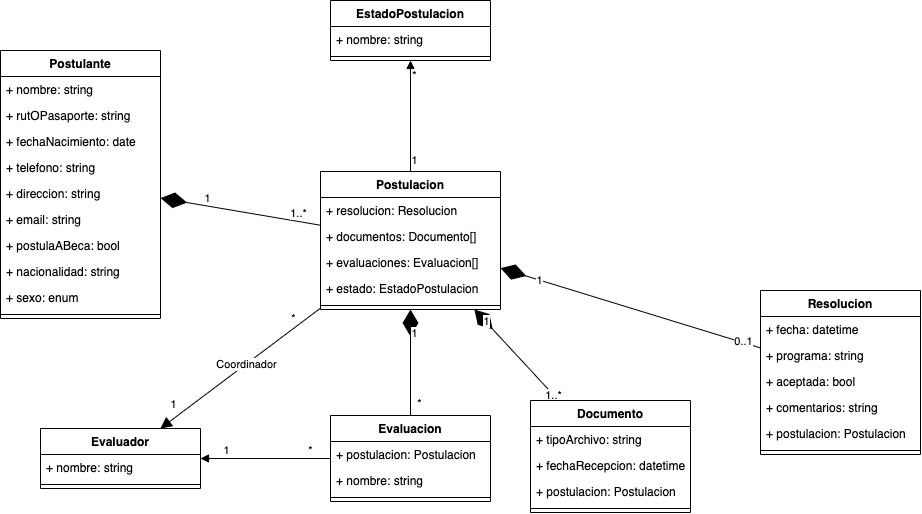
\includegraphics[scale=0.4]{imagenes/03-modelo-dominio.png}
    \end{center}
    \caption{Modelo de dominio del sistema}
    \label{fig:modelo-dominio}
\end{figure}

\section{Arquitectura del Sistema}

La Figura \ref{fig:arquitectura} muestra el modelo de contexto de la aplicación,
el cual representa el nivel de abstracción más alto en la representación de
arquitecturas según el modelo C4 [9]. Como se puede ver, los usuarios
interactúan con el sistema de evaluación de postulaciones al MTI, el cual extrae
los datos desde la aplicación web de UCampus. Esta arquitectura permite
independizar la forma de extraer datos, ya sea que esto se haga a través de una
API o a través de scrapers. El proceso de extracción de datos está encapsulado
un único módulo del sistema, lo cual permite reemplazarlo en caso de que a
futuro aparezcan mejores opciones para realizar la alimentación de datos.

\begin{figure}[!ht]
    \begin{center}
        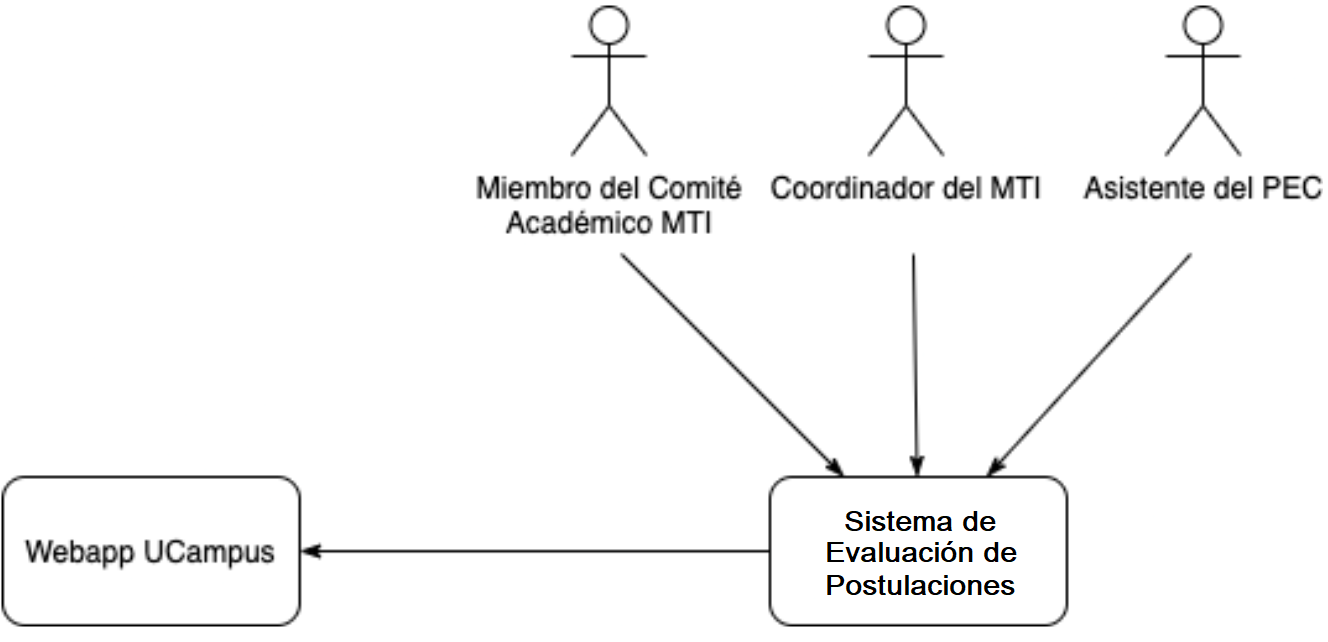
\includegraphics[scale=0.2]{imagenes/03-arquitectura.png}
    \end{center}
    \caption{Arquitectura general de la aplicación (Modelo de Contexto)}
    \label{fig:arquitectura}
\end{figure}

La Figura \ref{fig:descomposicion-sistema} muestra cómo está estructurado el
sistema en términos de sus macro-componentes y el repositorio de datos.
Particularmente, los usuarios del sistema interactúan con una aplicación
front-end, la cual contiene todas las interfaces de usuario del sistema. Ésta no
contiene la lógica de negocio, pues su rol es presentar la interfaz de usuario,
pedir datos al back-end, y mostrarlos al usuario.

Por otra parte, el back-end del sistema es el encargado de mantener la lógica de
la aplicación. En él se describen todos los procesos de negocio, y es el
encargado de la comunicación entre la interfaz de usuario y la base de datos. El
back-end además se comunica con la aplicación web de UCampus y extrae los datos
desde la página Web de postulaciones. Este componente es uno de los puntos más
críticos, pues es el que mantiene toda la lógica del sistema, y por lo tanto, es
el que ayuda a optimizar el proceso de postulaciones.

% El display de estas figuras es un desastre... mejorar

\begin{figure}[!ht]
    \begin{center}
        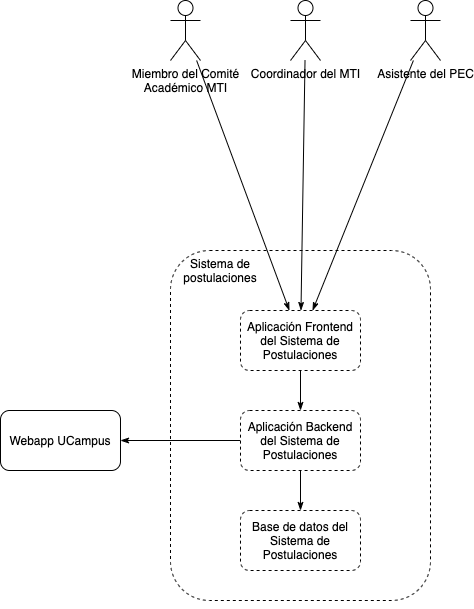
\includegraphics[scale=0.5]{imagenes/03-descomposicion-sistema.png}
    \end{center}
    \caption{Descomposición en componentes del Sistema de Evaluación de Postulaciones}
    \label{fig:descomposicion-sistema}
\end{figure}

Finalmente, la Figura \ref{fig:descomposicion-backend} muestra la descomposición
del back-end en sus principales componentes. Éste se divide en 4 componentes,
los cuales se describen a continuación.

\begin{figure}[!ht]
    \begin{center}
        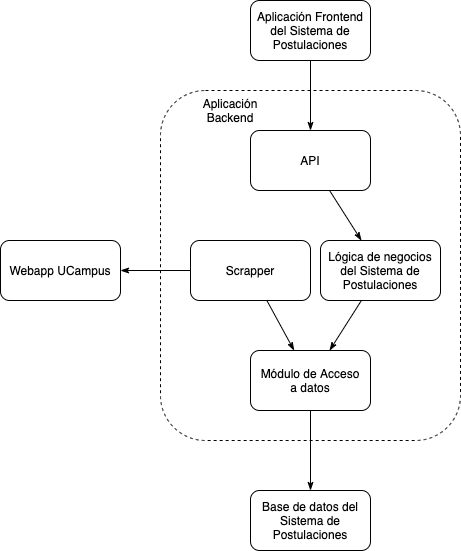
\includegraphics[scale=0.5]{imagenes/03-descomposicion-backend.png}
    \end{center}
    \caption{Descomposición en componentes del back-end del sistema (sólo se muestran los componentes relevantes).}
    \label{fig:descomposicion-backend}
\end{figure}

La \textbf{API} es un módulo HTTP encargado de disponibilizar los datos de la
aplicación para que puedan ser consumidos por la aplicación front-end. Este
módulo no contiene ninguna lógica; sólo sirve como medio de transporte de datos
desde y hacia la lógica de la aplicación. Por supuesto, este módulo también
recibe datos desde el front-end, y en dicho caso, es el encargado de transportar
esos datos hacia la capa de lógica de la aplicación.

Luego, el módulo de \textbf{lógica de negocios} es el encargado de implementar
el proceso y las interacciones de sus actores. En este módulo se puede encontrar
la lógica que procesa las postulaciones nuevas, crea las evaluaciones y recibe
los inputs de los actores del sistema.

El módulo de \textbf{acceso a datos} es el encargado de comunicarse con la base
de datos y persistir los datos que le llegan desde la lógica de negocio o desde
el scraper. Por último, el \textbf{scraper} es el módulo encargado de consumir
datos desde la página Web de UCampus, y enviarlos para que se almacenen en la
base de datos. Para ello, los datos que procesa el scraper son entregados como
input a la capa de acceso a datos. Vale la pena mencionar que los diagramas
antes presentados seguirán siendo válidos en el caso de que UCampus entregue los
datos de postulaciones vía una API para ser consumida por el sistema
desarrollado en esta memoria. La única cosa que cambiaría sería el uso de la
API, como reemplazo al actual uso del scraper.

\section{Modelo de Datos}

La figura \ref{fig:modelo-datos} muestra el modelo de datos del sistema, el cual
adhiere al modelo de dominio mostrado en la figura \ref{fig:modelo-dominio}.

\begin{figure}[!ht]
    \begin{center}
        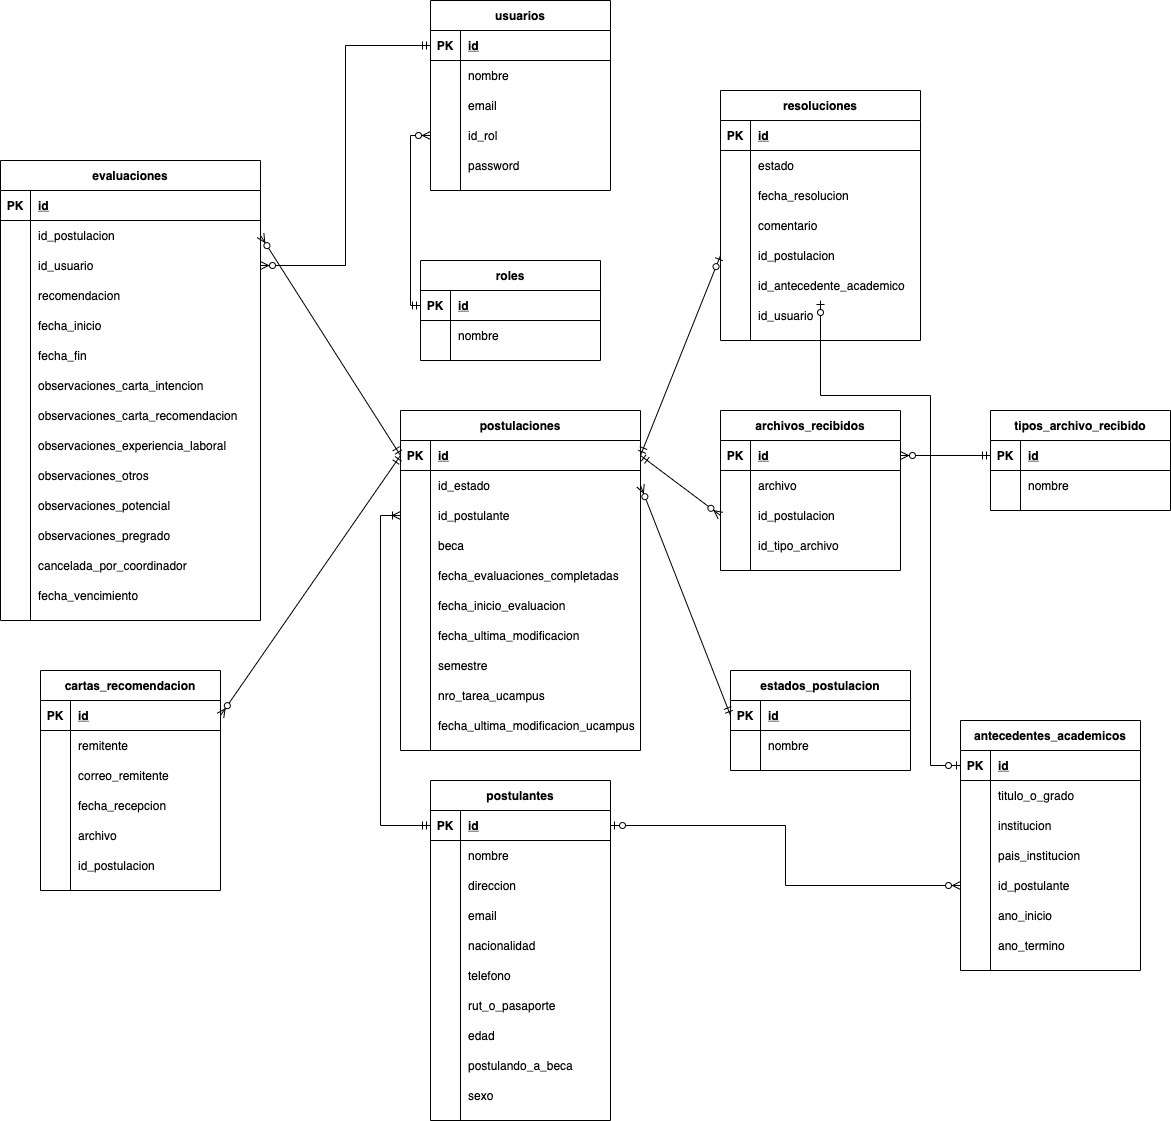
\includegraphics[scale=0.4]{imagenes/03-modelo-datos.png}
    \end{center}
    \caption{Modelo de datos del sistema}
    \label{fig:modelo-datos}
\end{figure}

En cada entidad de datos se puede ver los atributos de las mismas, cuyos nombres
son casi auto-explicativos. Tal como se ha mencionado antes, las postulaciones
son el centro neurálgico del sistema. Estas pertenecen a un postulante y tienen
documentación asociada (\texttt{cartas\_recomendacion} y
\texttt{archivos\_recibidos}, en Fig. \ref{fig:modelo-datos}). Además tienen
evaluaciones, un estado, y eventualmente resoluciones acerca de ellas, tal como
se indica en la figura. 

En el próximo capítulo se describe la implementación de este sistema.

\chapter{Implementación de la Solución}

La implementación de la solución cuenta con distintos módulos que usan distintas
tecnologías y potencialmente distintos lenguajes. Primero, para los módulos del
sistema se detallan las tecnologías escogidas, y luego se presentan las
interfaces creadas para los distintos actores (perfiles de usuario) del proceso.

\section{Tecnologías Escogidas para la Implementación}

En este apartado se describen los componentes críticos del sistema implementado,
y cuáles fueron las tecnologías usadas para tal propósito en cada caso. Antes de
eso, en todo caso, vale la pena explicar los requerimientos de implementación de
este sistema. Para ello, hay que tener muy claro qué capacidades tiene
actualmente la aplicación, cuál es su perspectiva de evolución a futuro, y cómo
será la operación de la misma. Estos tres puntos son claves para tomar cualquier
decisión con respecto a las tecnologías que se escojan para implementar el
sistema.

Primero que todo, este sistema muestra que se puede obtener datos desde UCampus
y usarlos para automatizar de forma interna el proceso de evaluación de las
postulaciones. Luego, el futuro de este sistema puede tomar dos rumbos: 1) los
datos se extraerán desde una API que exponga UCampus, o 2) la plataforma UCampus
estandariza el formulario de postulación a todos los programas de la Facultad
(hoy en día dicho formulario no está estandarizado). 

La segunda alternativa es poco viable en el corto plazo, pues requiere que todos
los programas de la Facultad se pongan de acuerdo acerca de qué información debe
aportar el postulante a la hora de postular a uno de ellos. Esto parece ser
difícil de alcanzar, pues muchos de estos programas tienen naturaleza distinta
(algunos tienen un perfil profesional y otros científico), y distintos niveles
de exigencia (por ejemplo, para magíster y doctorado).

Considerando estos aspectos, el sistema de evaluación de postulaciones debe
estar preparado para el futuro de varias formas: 

\begin{itemize}
\item Debe ser extensible, en el sentido de que debe permitir cambiar el método
de extracción de datos de las postulaciones.
\item Debe ser altamente mantenible, pues hay componentes que su actual
implementación depende de componentes o condiciones externas, que podrían
cambiar en un futuro inmediato. A pesar de eso el sistema debería poder
adaptarse en forma rápida para seguir brindando el servicio.
\item La operación de este sistema debe presentar la menor cantidad de
impedimentos, y bloqueos técnicos posibles, tanto para los desarrolladores como
para los administradores de sistemas.
\end{itemize}

A continuación se explican las tecnologías que se utilizaron para implementar
los macro-componentes de este sistema.

\subsection{Back-end}

El back-end es la piedra angular de esta aplicación. Dentro de él, funcionan el
scraper, la conexión a la base de datos y la disponibilización de los datos de
forma segura. Para implementar el back-end, la primera restricción es que
presenta, es que existen dos maneras viables para extraer los datos de las
postulaciones desde UCampus; cada una con su propio entorno de desarrollo. Una
de ellas usa Node.js, y otra está en Python.

Para tomar esta decisión, la Stack Overflow Developer Survey 2020 [10] reveló
que Python es el tercer lenguaje más amado por desarrolladores, sólo superado
por TypeScript y Rust. Python es además el lenguaje que más desarrolladores
buscan aprender.

A pesar de lo antes mencionado, sigue estando la opción de usar Puppeteer [3]
con TypeScript para implementar el back-end. Sin embargo, teniendo en cuenta el
perfil de los potenciales desarrolladores que tendrá el sistema, el uso de
Python parece ser la opción más apropiada para implementar el back-end del
sistema. Python es un lenguaje que cualquier estudiante de una Universidad
chilena conoce, al contrario de TypeScript, que si bien es un lenguaje con mucha
popularidad en la industria, no lo es tanto en el mundo académico.

Por las razones mencionadas anteriormente, el lenguaje escogido para escribir el
back-end es Python. Dado eso, queda por decidir cómo conectarse a la base de
datos, y cómo exponer los datos de las postulaciones de forma segura.


\subsubsection{Base de Datos}

La encuesta a desarrolladores mencionada anteriormente (de Stack Overflow)
mostró que PostgreSQL es la base de datos persistente más amada por estas
personas [10]. Le siguen, en orden, Elastic Search y MongoDB. Por otro lado,
PostgreSQL es la segunda base de datos que los desarrolladores buscan aprender,
sólo precedida por MongoDB.

La base de datos rankeada como \#1 en la encuesta es Redis [12]; sin embargo,
ésta no es una opción puesto que es una base de datos en memoria.

Con respecto a bases de datos SQL (PostgreSQL) y NoSQL (Elastic Search y
MongoDB), la naturaleza estructurada y relacional de los datos existentes hacen
que inclinarse por PostgreSQL sea una buena idea. Otra razón para ello es que
potenciales desarrolladores de este sistema muy probablemente no estarán muy
familiarizados con bases de datos NoSQL, pues son menos abordadas en cursos
bases de datos a nivel de pregrado. Por las razones anteriormente expuestas, se
decidió que los datos de este sistema se almacenen en una base de datos
PostgreSQL.

\subsubsection{Servidor HTTP}

Para el servidor HTTP se deben tomar en cuenta las siguiente consideraciones:

\begin{itemize}
\item Rendimiento (performance) del servidor, medido en cantidad de respuestas
por segundo.
\item Curva de aprendizaje para nuevos desarrolladores.
\end{itemize}

% ref tabla
Para evaluar el rendimiento potencial del servidor se analizó la información
disponible en the benchmarker [11], el cual consta de una serie de repositorios
dedicados a encontrar benchmarks de servidores HTTP en frameworks web. Para cada
framework se mide la cantidad de respuestas por segundo, según la cantidad de
threads concurrentes que intentan acceder al servidor. En la Tabla
\ref{table:frameworks} se muestra un resumen de los resultados obtenidos por los
frameworks más conocidos.

\begin{table}[!ht]
    \begin{center}
        \begin{tabular}{|l|l|l|r|r|r|}
            \hline
            \# & Lenguaje & Framework & Req/s (64) & Req/s (128) & Req/s (256) \\ \hline
            58 & python (3.9) & falcon (2.0) & 74.256,04 & 81.538,76 & 82.897,69 \\ \hline
            88 & python (3.9) & pyramid (2.0) & 51.298,30 & 56.850,32 & 57.128,55 \\ \hline
            100 & python (3.9) & asgineer (0.8) & 44.745,54 & 51.318,30 & 52.105,43 \\ \hline
            104 & python (3.9) & bottle (0.12) & 39.690,41 & 42.590,65 & 44.329,21 \\ \hline
            107 & python (3.9) & emmett (2.2) & 35.983,95 & 41.270,86 & 42.295,95 \\ \hline
            115 & python (3.9) & apidaora (0.28) & 34.119,60 & 38.263,87 & 38.707,73 \\ \hline
            116 & python (3.9) & hug (2.6) & 34.040,91 & 35.909,39 & 53.828,77 \\ \hline
            125 & python (3.9) & blacksheep (1.0) & 28.887,22 & 33.204,44 & 34.356,25 \\ \hline
            129 & python (3.9) & index.py (0.16) & 27.273,81 & 29.282,48 & 30.258,63 \\ \hline
            131 & python (3.9) & starlette (0.14) & 26.693,66 & 31.709,52 & 31.302,99 \\ \hline
            134 & python (3.9) & responder (2.0) & 26.092,65 & 31.092,58 & 32.175,53 \\ \hline
            135 & python (3.9) & clastic (199) & 25.651,88 & 28.936,99 & 28.781,05 \\ \hline
            136 & python (3.9) & sanic (21.3) & 25.446,08 & 28.833,98 & 29.194,50 \\ \hline
            145 & python (3.9) & molten (1.0) & 18.055,01 & 21.858,74 & 21.906,60 \\ \hline
            146 & python (3.9) & aiohttp (3.7) & 17.837,07 & 23.359,98 & 24.128,26 \\ \hline
            149 & python (3.9) & fastapi (0.63) & 16.701,72 & 22.402,72 & 22.042,29 \\ \hline
            164 & python (3.9) & flask (1.1) & 12.901,82 & 16.427,23 & 16.521,94 \\ \hline
            176 & python (3.9) & cherrypy (18.6) & 9.328,09 & 9.396,33 & 8.832,55 \\ \hline
            177 & python (3.9) & guillotina (6.2) & 9.152,33 & 8.843,65 & 8.742,31 \\ \hline
            181 & python (3.9) & quart (0.14) & 7.571,28 & 7.501,08 & 6.888,88 \\ \hline
            183 & python (3.9) & tonberry (0.2) & 7.363,12 & 6.948,61 & 6.344,40 \\ \hline
            191 & python (3.9) & django (3.1) & 5.918,73 & 6.572,13 & 6.150,29 \\ \hline
            193 & python (3.9) & tornado (6.1) & 5.722,03 & 5.728,67 & 5.624,07 \\ \hline
            210 & python (3.9) & masonite (3.0) & 2.485,30 & 2.477,63 & 2.477,29 \\ \hline
            217 & python (3.9) & cyclone (1.3) & 1.597,57 & 1.591,42 & 1.577,40 \\ \hline
            218 & python (3.9) & klein (20.6) & 1.501,11 & 1.538,24 & 1.513,71 \\ \hline
            220 & python (3.9) & nameko (2.13) & 1.213,25 & 1.164,90 & 1.142,60 \\ \hline
            222 & python (3.9) & django-ninja (0.11) & 1.065,37 & 1.478,17 & 1.496,42 \\ \hline
        \end{tabular}
    \end{center}
    \caption{Rendimiento de frameworks de Python. La primera columna indica la posición entre todos los frameworks testeados y desde la cuarta columna en adelante, el número representa la cantidad promedio de peticiones completadas por segundo para una cierta cantidad de clientes haciendo estas peticiones concurrentemente (el número indicado en paréntesis)}
    \label{table:frameworks}
\end{table}

La Tabla \ref{table:frameworks} muestra los resultados para herramientas python
que sirven para implementar el back-end del sistema. Las columnas de resultados
(que parten con \emph{Req/s}) indican cuántas peticiones por segundo puede
responder el servidor cuando hay una cierta cantidad de usuarios haciendo
peticiones de forma concurrente (el número entre los paréntesis).

En todo caso, hay que tener en cuenta que muchas de estas herramientas suelen
ser experimentales, y otras son tan minimales que no es viable su uso para
sistemas como el reportado en esta memoria.

Tomando en cuenta la popularidad de los paquetes, en término de cantidad de
estrellas en GitHub, los contendores son:

\begin{itemize}
    \item FastAPI (29.2k estrellas)
    \item Django (56.5k estrellas)
    \item Flask (54.4k estrellas)
\end{itemize}

FastAPI es el más nuevo de los tres y cuenta con soporte para asyncio [14], con
tutoriales cortos donde se explica la totalidad de sus capacidades. Django es el
más popular, con una gran cantidad de capacidades (tan grande de hecho, que no
se hacen necesarias todas ellas). Finalmente, Flask es prácticamente FastAPI,
pero sin soporte para asyncio, ni inyección de dependencias.

Considerando lo anterior, se decidió utilizar usar FastAPI tomando en cuenta
diversos aspectos:

\begin{itemize}
    \item Su gran popularidad pese a su poco tiempo de vida, comparado con Flask
    y Django.
    \item Soporta asyncio en forma nativa. El uso de asyncio hace que pueda
    manejar una mayor cantidad de peticiones por segundo.
    \item La barrera de entrada para usar este framework es mucho más pequeña
    que Django y es comparable a Flask. Por lo tanto, para el futuro de este
    proyecto, los nuevos desarrolladores no tendrán que entender la filosofía de
    un framework completo, como Django, sino que simplemente les bastará
    entender cómo funcionan los módulos de Python.
\end{itemize}

\subsection{Scraper}

Con respecto al scraper, ya se introdujo anteriormente las alternativas
evaluadas, estas eran: Puppeteer [3] y Selenium [4]. Al tomar en cuenta que
Selenium tiene bindings para Python, se hace evidente usarlo en vez de
Puppeteer. De nuevo, la mantenibilidad juega un rol importante en esta decisión.

\subsection{Deployment}

Para decidir cómo hacer el deployment de la aplicación, se tuvo en cuenta que el
sistema involucra, entre otros:

\begin{enumerate}
    \item Un módulo de scraping, que requiere ejecutables en el sistema
    operativo host.
    \item Una API.
    \item Ejecución continua del módulo de scraping.
\end{enumerate}

La instalación de un sistema con tales características no es trivial, pues no
sólo se necesita de las dependencias naturales de Python, sino además
componentes del sistema operativo para que funcione.

Para automatizar esa tarea y hacer el deployment de esta aplicación un proceso
confiable, Docker [13] es una herramienta que permite abstraer tales
restricciones y hace del deployment un proceso con bajo riesgo, pues no importa
el ambiente en el que se ejecuta el proyecto. En ese sentido, sólo basta que
funcione en Docker.

\subsection{Front-end}

Con respecto al front-end, los dos lenguajes más populares para implementar un
sitio web con sus interfaces son JavaScript y TypeScript. Existen otras opciones
que simplemente se descartan por baja popularidad, y por lo tanto, una
potencialmente baja capacidad para darle mantenimiento al sistema.

El Developer Survey 2020 de Stack Overflow [11] reveló que, de los frameworks
web más apreciados por los desarrolladores, React [15] está en la posición 2,
mientras que Vue.js [16] está en la posición 3; ambos superados por ASP.NET
Core, que se descarta usar en este proyecto simplemente porque requiere que el
servidor sea escrito en C\#, lenguaje que no es opción para este proyecto.

React [15] es el framework JavaScript más popular de front-end en el mercado, y
es elegido para el desarrollo de esta aplicación precisamente por eso. Como en
este proyecto se prioriza la mantenibilidad, React es probablemente la mejor
opción. Vue [16] es el segundo framework más popular. Sin embargo, al momento
del comienzo de la implementación de este sistema, Vue se encontraba en
transición entre la versión 2 a la 3. Por lo tanto, elegirlo habría implicado
trabajar con APIs inestables, o bien con APIs obsoletas. Por las razones
anteriormente expuestas, React es la opción elegida para este proyecto.

\section{Interfaces de Usuario}

En esta sección se presentan las principales interfaces de usuario del sistema.
El propósito de esto es ilustrar cómo se ayuda a los diferentes tipos de
usuario, a cumplir con sus tareas. Para evitar la sobre extensión del documento,
sólo se muestran las principales interfaces para cada usuario; es decir, sólo
aquellas que son críticas para el cumplimiento de las funciones asignadas a cada
rol.

En primer lugar se muestra la interfaz principal del sistema, a la cual se
accede luego del proceso de autenticación del usuario (Figura 8). En este caso
el usuario está logueado con el rol de asistente. Es importante aclarar que los
datos mostrados en estas interfaces son ficticios.

\begin{figure}[!ht]
    \begin{center}
        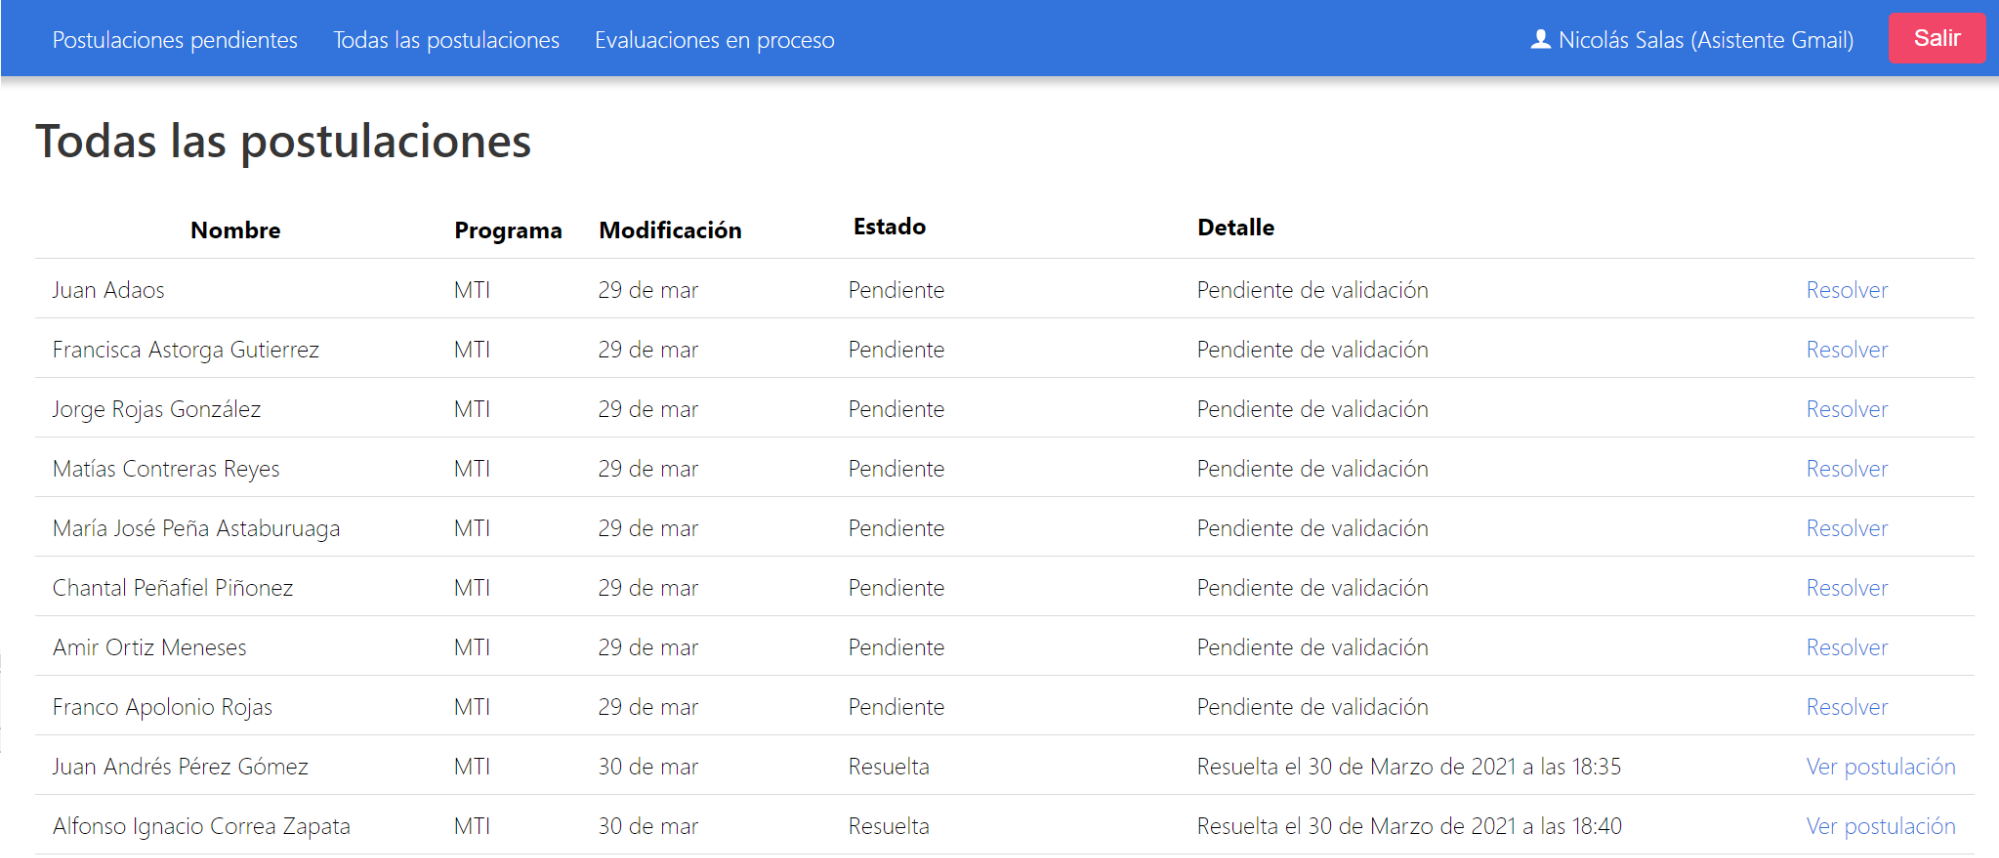
\includegraphics[scale=0.23]{imagenes/04-interfaz-principal.png}
    \end{center}
    \caption{Interfaz principal del sistema}
    \label{fig:interfaz-principal}
\end{figure}

El menú principal tiene tres opciones: postulaciones pendientes, todas las
postulaciones y postulaciones en proceso. La semántica de cada categoría varía
dependiendo del perfil de usuario que accede a la información. En el caso de la
Figura \ref{fig:interfaz-principal}, la información que se muestra corresponde a
“todas las postulaciones”, esto incluye las “pendientes de evaluación”, las “en
proceso” y las “resueltas”. A continuación se explican las principales
interfaces para cada rol.

\subsection{Interfaces de Usuario para el Asistente}

En el caso del usuario asistente, las postulaciones pendientes corresponden a
aquellas que aún no han sido mandadas a evaluar (Figura
\ref{fig:interfaz-pendientes}), probablemente porque aún no tienen todos los
documentos que se requiere para poder procesarlas. Para verificar esto, el
asistente debe clickear en el link “Resolver” de la postulación que quiere
revisar. Una vez hecho eso, accede a la postulación.

\begin{figure}[!ht]
    \begin{center}
        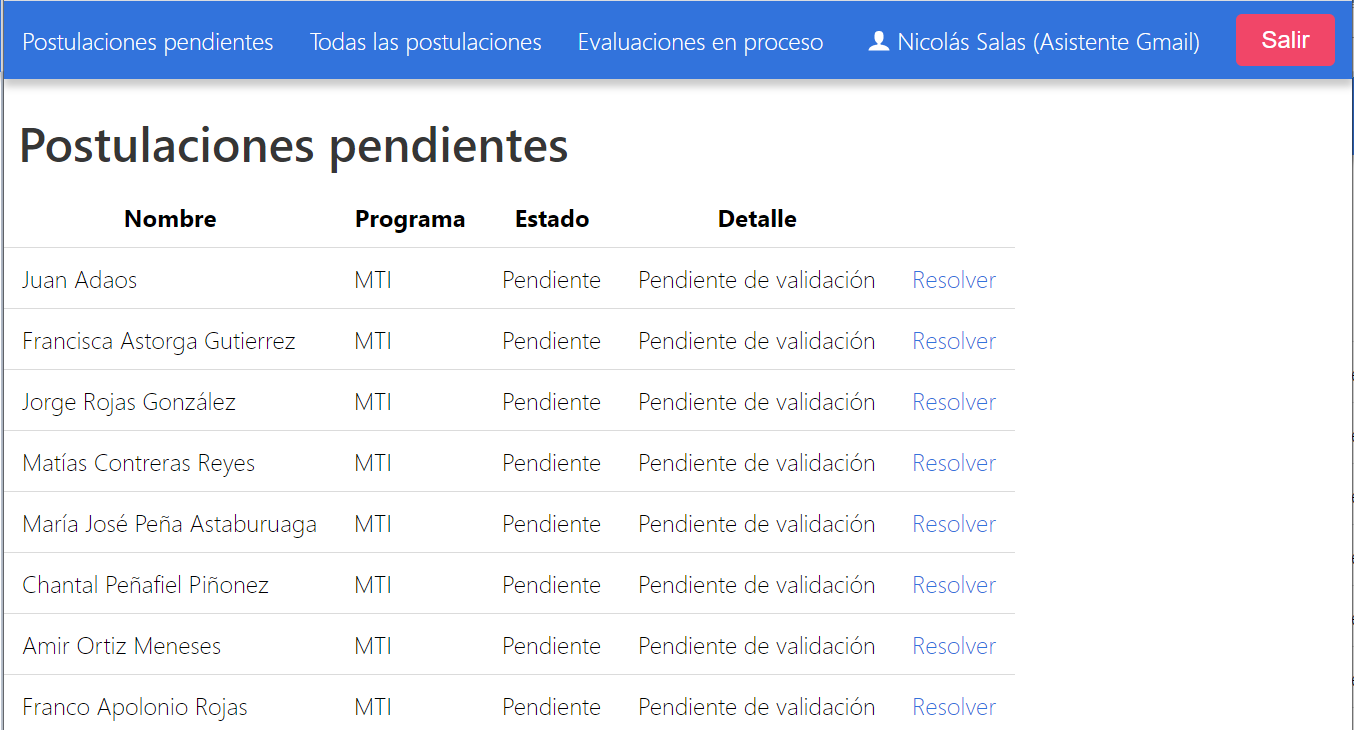
\includegraphics[scale=0.23]{imagenes/04-interfaz-pendientes.png}
    \end{center}
    \caption{Interfaz de postulaciones pendientes}
    \label{fig:interfaz-pendientes}
\end{figure}

La figura \ref{fig:formulario-antecedentes} muestra cómo se ven los datos de una
postulación para un usuario asistente. A la izquierda se muestran los datos
personales del postulante, que han sido ofuscados por temas de privacidad. En la
sección media de la interfaz se presentan los antecedentes académicos del
postulante, y a la derecha se encuentran los documentos requeridos por el
programa para que sea válida una postulación. Los documentos que han sido
subidos correctamente contienen un link; éste sirve para descargar dicho
documento y verificar que corresponde a lo requerido (por ejemplo, es un
Currículum Vitae). Los documentos que aparecen en rojo son aquellos que están
faltantes.

\begin{figure}[!ht]
    \begin{center}
        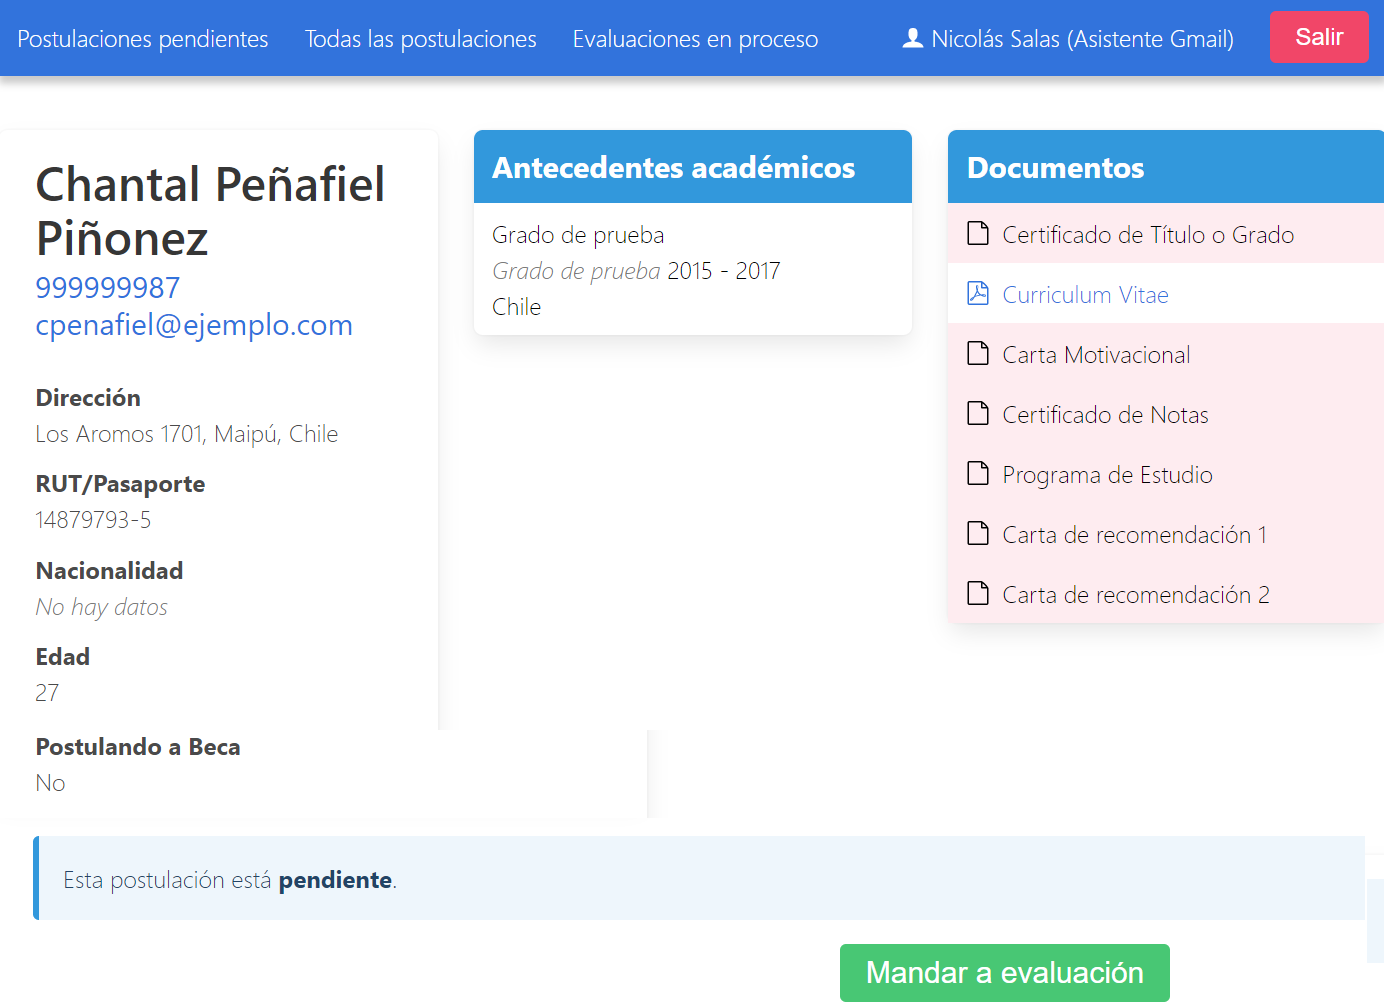
\includegraphics[scale=0.23]{imagenes/04-antecedentes-postulacion.png}
    \end{center}
    \caption{Formulario de antecedentes de la postulación}
    \label{fig:formulario-antecedentes}
\end{figure}

Aunque la postulación no tenga todos los datos que considera el formulario, ésta
se puede mandar a evaluar si tiene lo mínimo necesario. Para ello, al hacer
click en el botón “Mandar a Evaluación” (Figura
\ref{fig:formulario-antecedentes}), el sistema le informa al usuario el estado
de completitud de la postulación, y le pide confirmar la acción antes indicada
(Figura \ref{fig:confirmacion-evaluacion}).

\begin{figure}[!ht]
    \begin{center}
        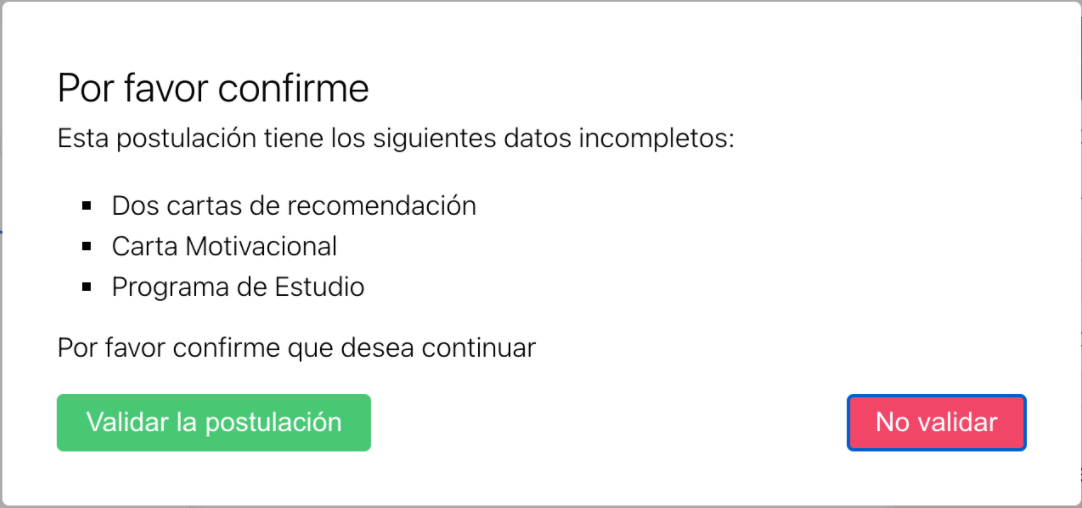
\includegraphics[scale=0.23]{imagenes/04-confirmacion-evaluacion.png}
    \end{center}
    \caption{Confirmación al mandar una postulación a evaluación}
    \label{fig:confirmacion-evaluacion}
\end{figure}

La opción “evaluaciones en proceso” para este perfil de usuario, al igual que
para el perfil coordinador, muestra las postulaciones que han sido enviadas a
evaluar y que aún no cuentan con una resolución por parte del coordinador. La
opción “todas las evaluaciones” muestra lo ya indicado en la figura
\ref{fig:interfaz-pendientes}.

\subsection{Interfaces de usuario para los Evaluadores}

Las interfaces de los usuarios evaluadores son similares a la de los usuarios
asistentes en términos de estructura e información mostrada. Sin embargo, los
evaluadores sólo pueden ver la información de las postulaciones asignadas a
ellos, mientras que los asistentes pueden ver todas las postulaciones.

Otra diferencia radica en la semántica de la opción de menú “evaluaciones
pendientes”, que en el caso de los evaluadores corresponde a las postulaciones
asignadas a ellos, pero sobre las cuales aún no emiten un juicio de aceptación o
rechazo.

Una tercera diferencia corresponde a que este perfil de usuario puede evaluar
una postulación, y para ello debe completar el formulario que se muestra en la
figura \ref{fig:formulario-evaluacion}. Los campos del formulario completo se
muestran en el Anexo B.

\begin{figure}[!ht]
    \begin{center}
        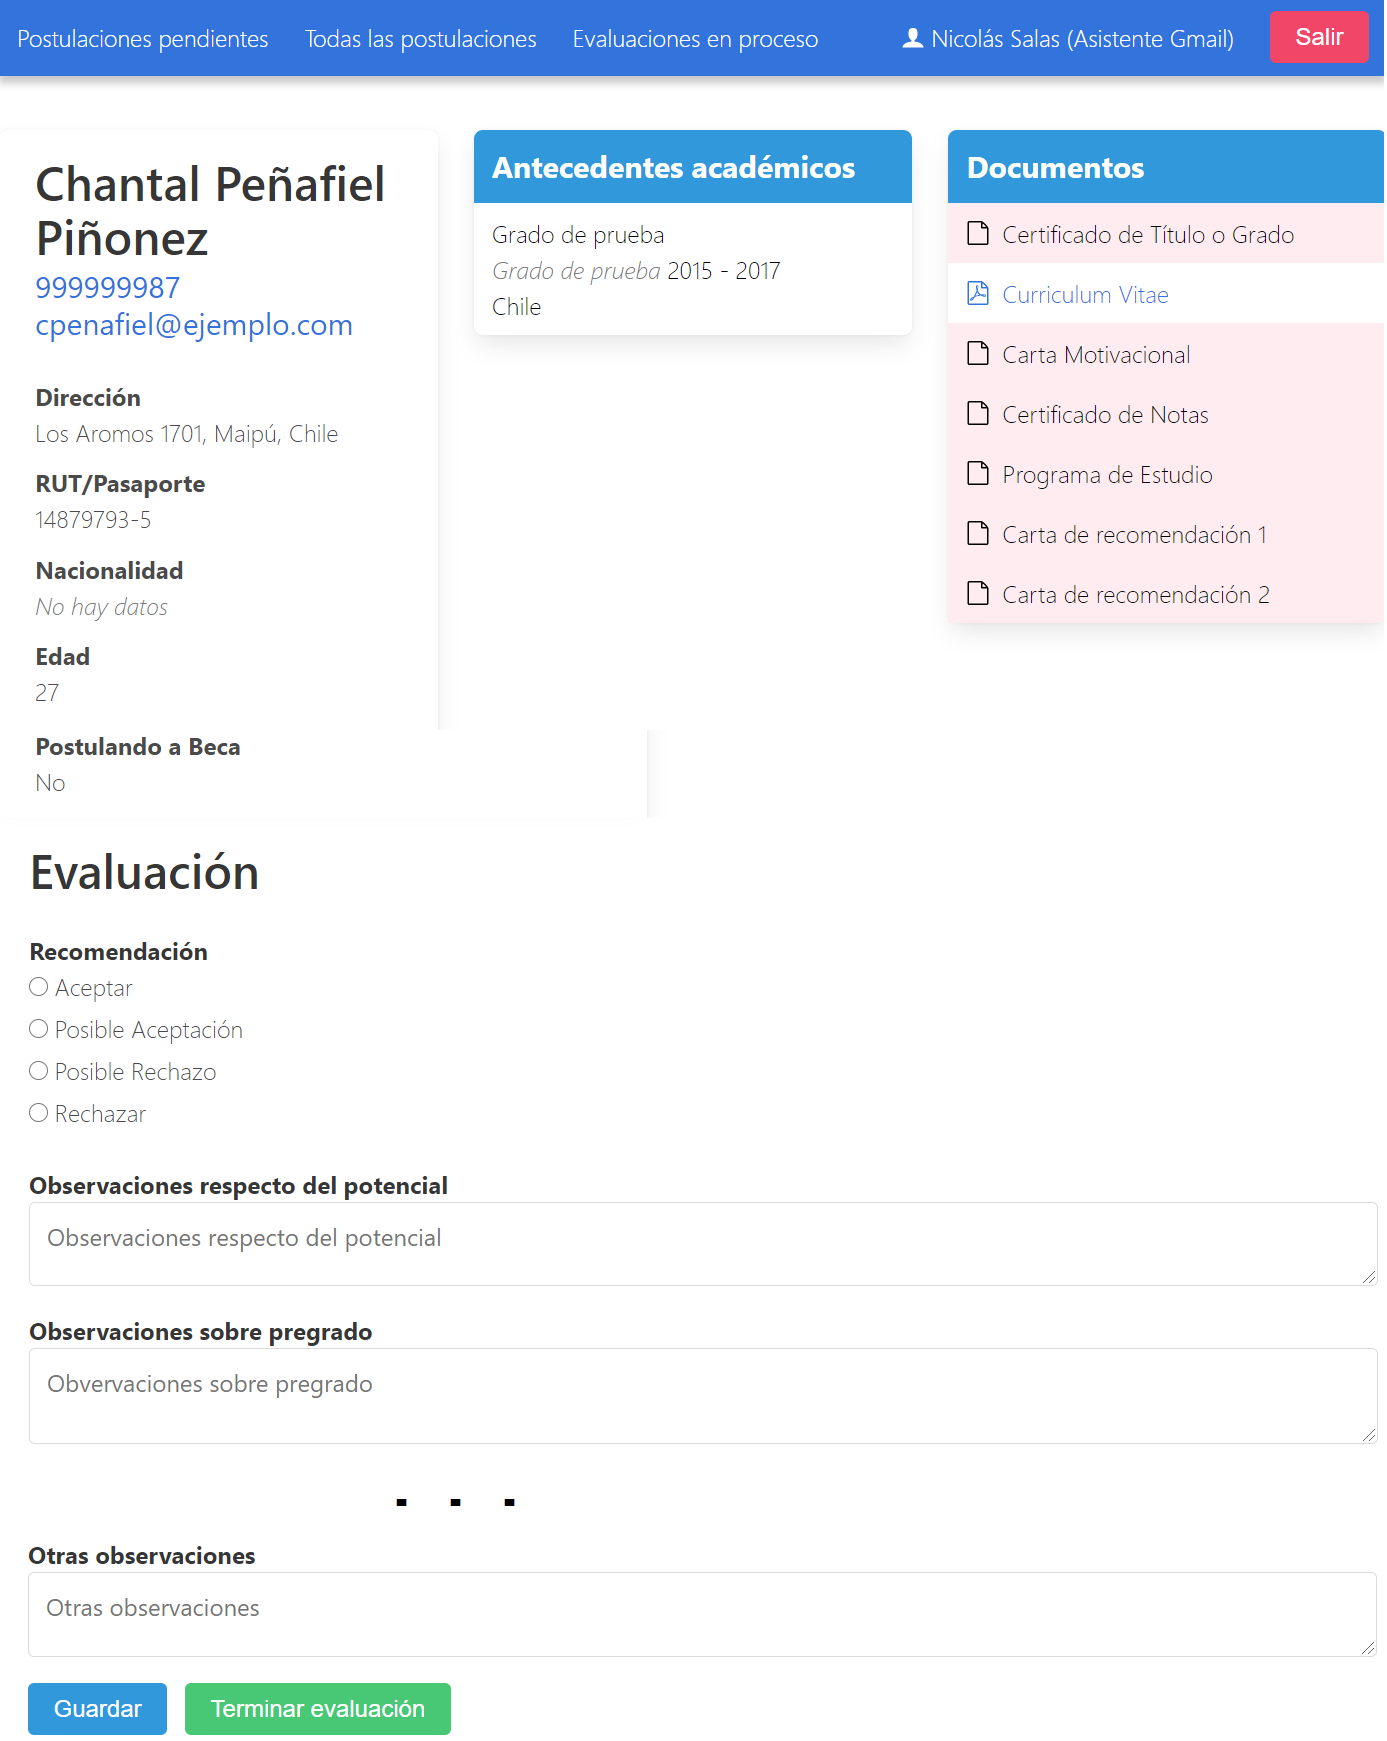
\includegraphics[scale=0.33]{imagenes/04-formulario-evaluacion.png}
    \end{center}
    \caption{Formulario de evaluación de una postulación}
    \label{fig:formulario-evaluacion}
\end{figure}

Una cuarta diferencia entre las interfaces de los evaluadores y los asistentes
consiste en que los primeros, una vez que han emitido su opinión, pueden acceder
a las opiniones emitidas por otros miembros del comité académico. Los asistentes
no tienen acceso a los comentarios de los evaluadores.

\subsection{Interfaces de Usuario para el Coordinador}

Al igual que en los casos anteriores, la opción de menú “Postulaciones
pendientes” muestra todas aquellas postulaciones sobre las cuales el coordinador
tiene algo pendiente (una acción que tomar). En la figura
\ref{fig:pendientes-coordinador} se muestran postulaciones en estado “pendiente
de validación”, las cuales corresponden a aquellas que aún no se han mandado a
evaluar. También se muestran las que están“en evaluación por el comité
académico”, y finalmente, aquellas que están esperando una resolución por parte
del usuario coordinador.

\begin{figure}[!ht]
    \begin{center}
        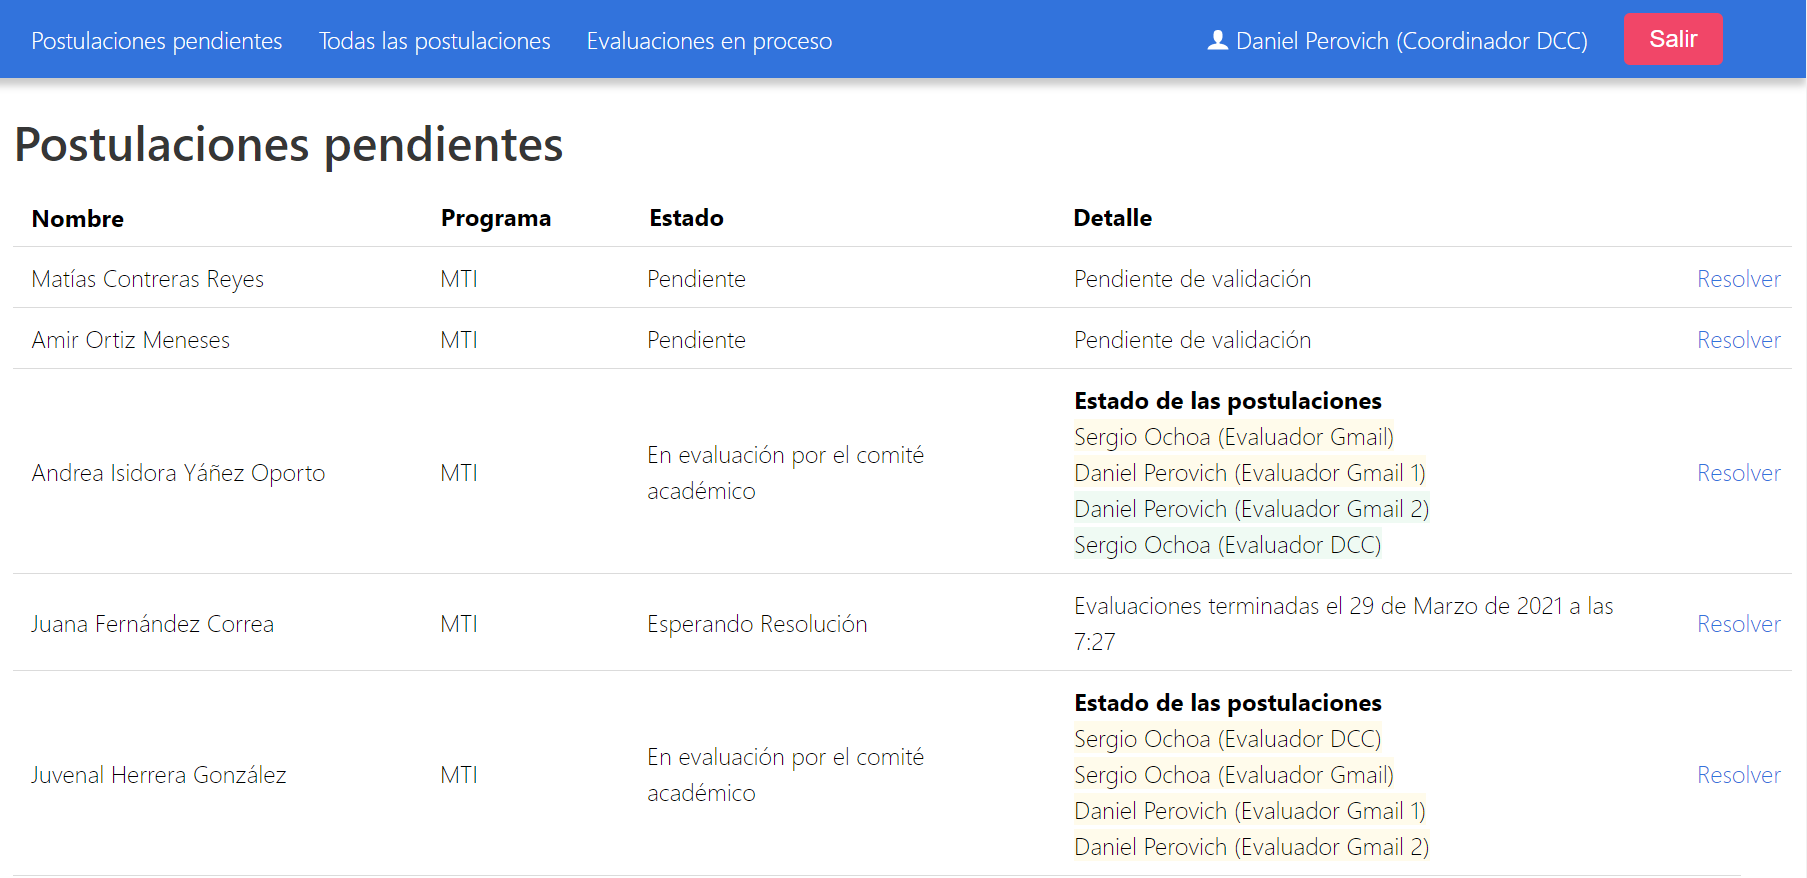
\includegraphics[scale=0.23]{imagenes/04-pendientes-coordinador.png}
    \end{center}
    \caption{Postulaciones pendientes para un usuario coordinador}
    \label{fig:pendientes-coordinador}
\end{figure}

Una vez que una postulación cuenta con la opinión de tres o más evaluadores, el
coordinador puede acceder y resolver sobre la aceptación o rechazo del
postulante. En la Figura \ref{fig:pendientes-coordinador}, la cuarta postulación
se encuentra en ese estado. Para tomar una decisión el coordinador clickear en
“Resolver” y accede al formulario que se muestra en la Figura
\ref{fig:resolucion} (vista parcial del formulario real).

\begin{figure}[!ht]
    \begin{center}
        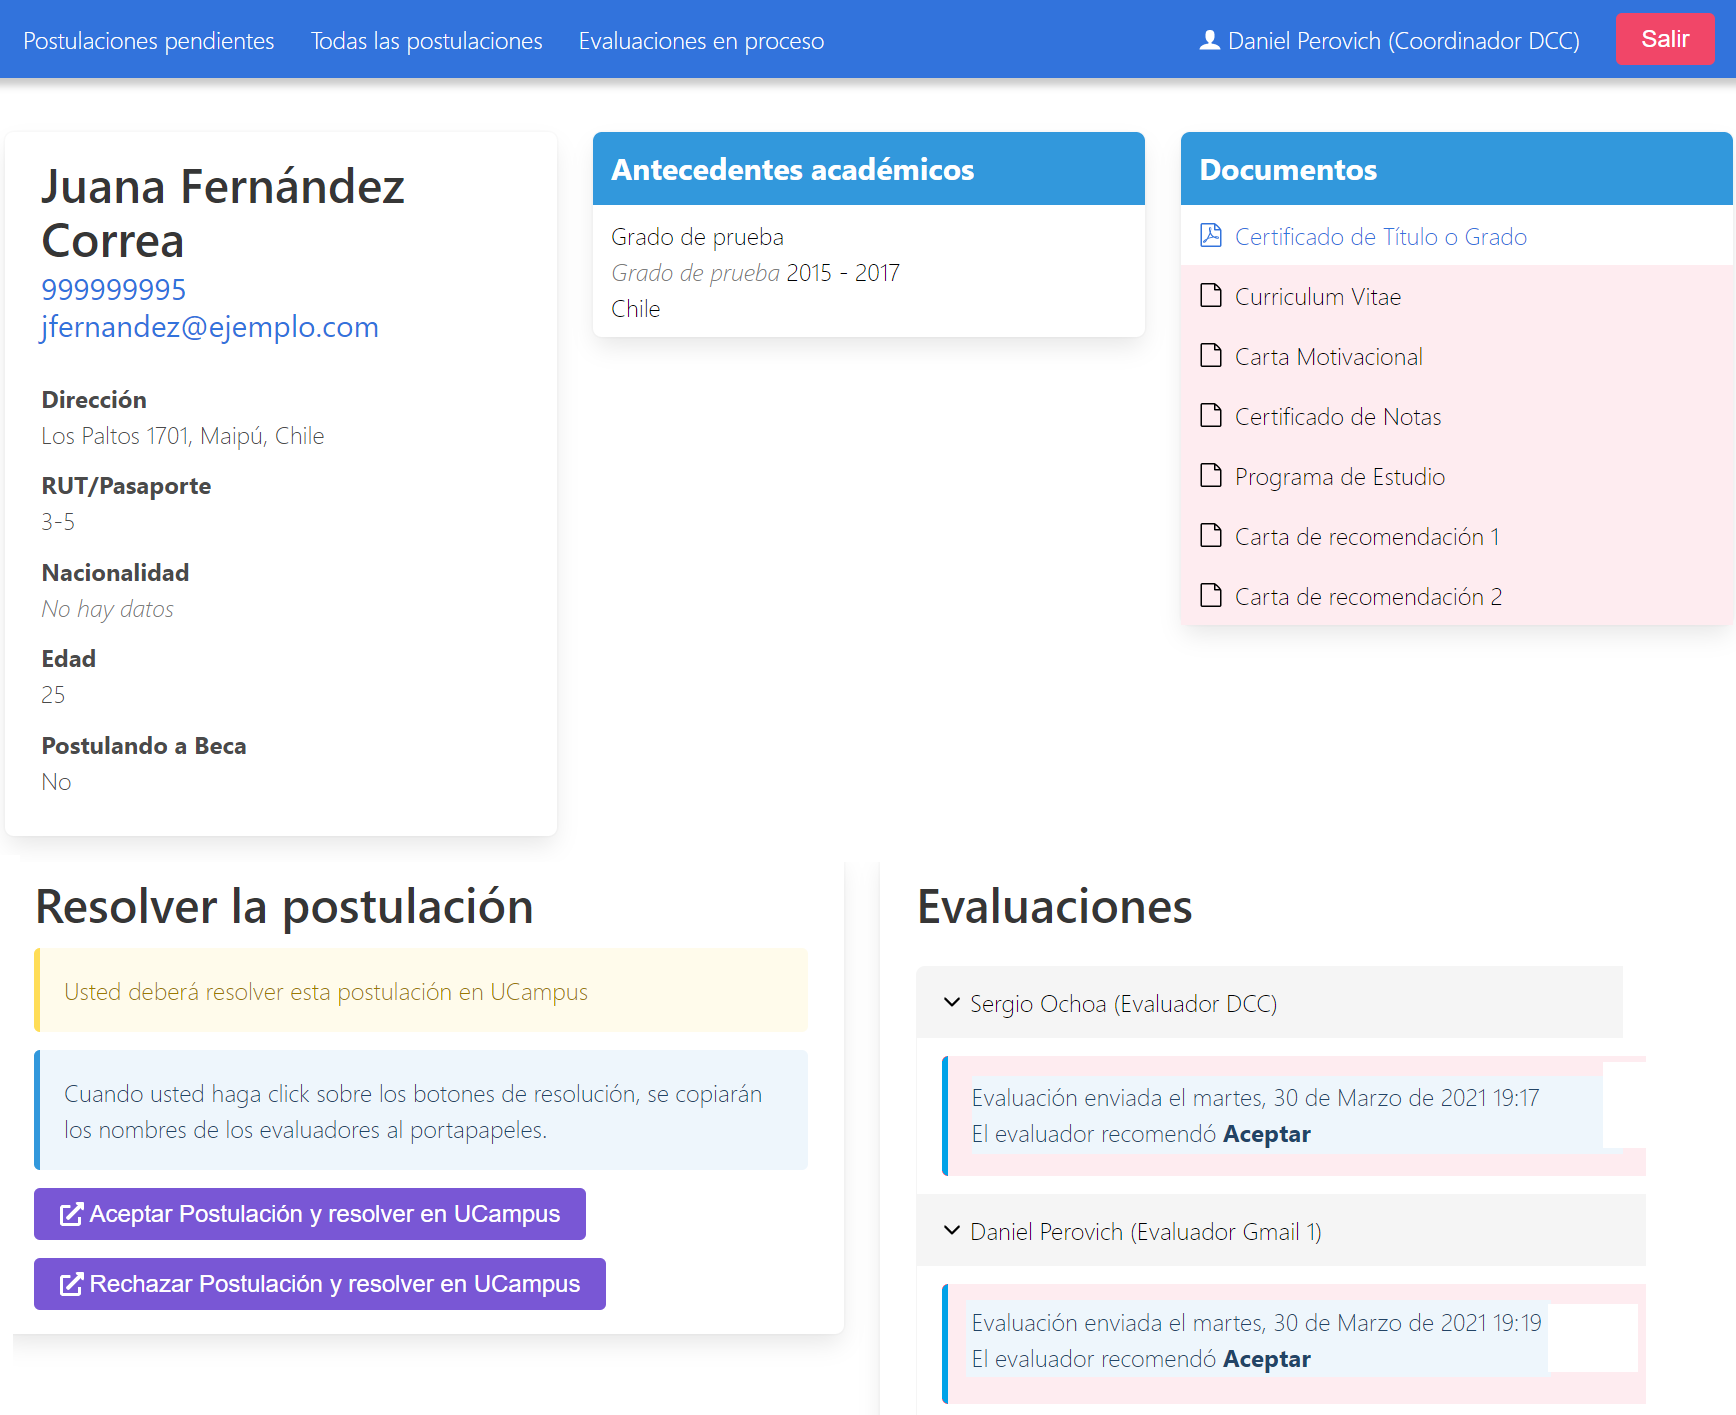
\includegraphics[scale=0.23]{imagenes/04-resolucion.png}
    \end{center}
    \caption{Formulario de resolución de postulaciones}
    \label{fig:resolucion}
\end{figure}

Para terminar, una vez que el coordinador emite su evaluación sobre el
postulante, la postulación avanza al estado “Esperando Resolución”. En este
estado, el coordinador debe resolver si acepta o rechaza la postulación. Para
ello, la figura \ref{fig:resolucion} muestra dos botones en el lado izquierdo de
la interfaz, uno para aceptar y otro para rechazar la postulación. Al lado
derecho en dicha interfaz se muestran las evaluaciones y recomendaciones de cada
evaluador.

Sea cual sea la decisión del coordinador, en el momento en que se presiona
cualquiera de los botones, se termina el proceso interno de evaluación de una
postulación, y ésta debe resolverse en UCampus. Esto es porque a pesar de que el
sistema marque la postulación como resuelta, UCampus no expone una forma de
resolver postulaciones, y por dicha razón, se debe resolver la postulación
dentro de UCampus.

Mientras tanto, el sistema internamente marca la postulación como resuelta.
Cuando una postulación ya está resuelta internamente en el sistema de evaluación
de postulaciones, el coordinador verá la interfaz mostrada en la figura
\ref{fig:postulacion-resuelta}, la que le permite (en caso de ser necesario)
devolver la postulación al estado “Esperando Resolución”. Esto se hace
clickeando el botón “Volver a evaluación”. La razón de esta interfaz es para
poder mitigar posibles equivocaciones del coordinador, al momento de presionar
los botones que indican la aceptación o rechazo de una postulación.

\begin{figure}[!ht]
    \begin{center}
        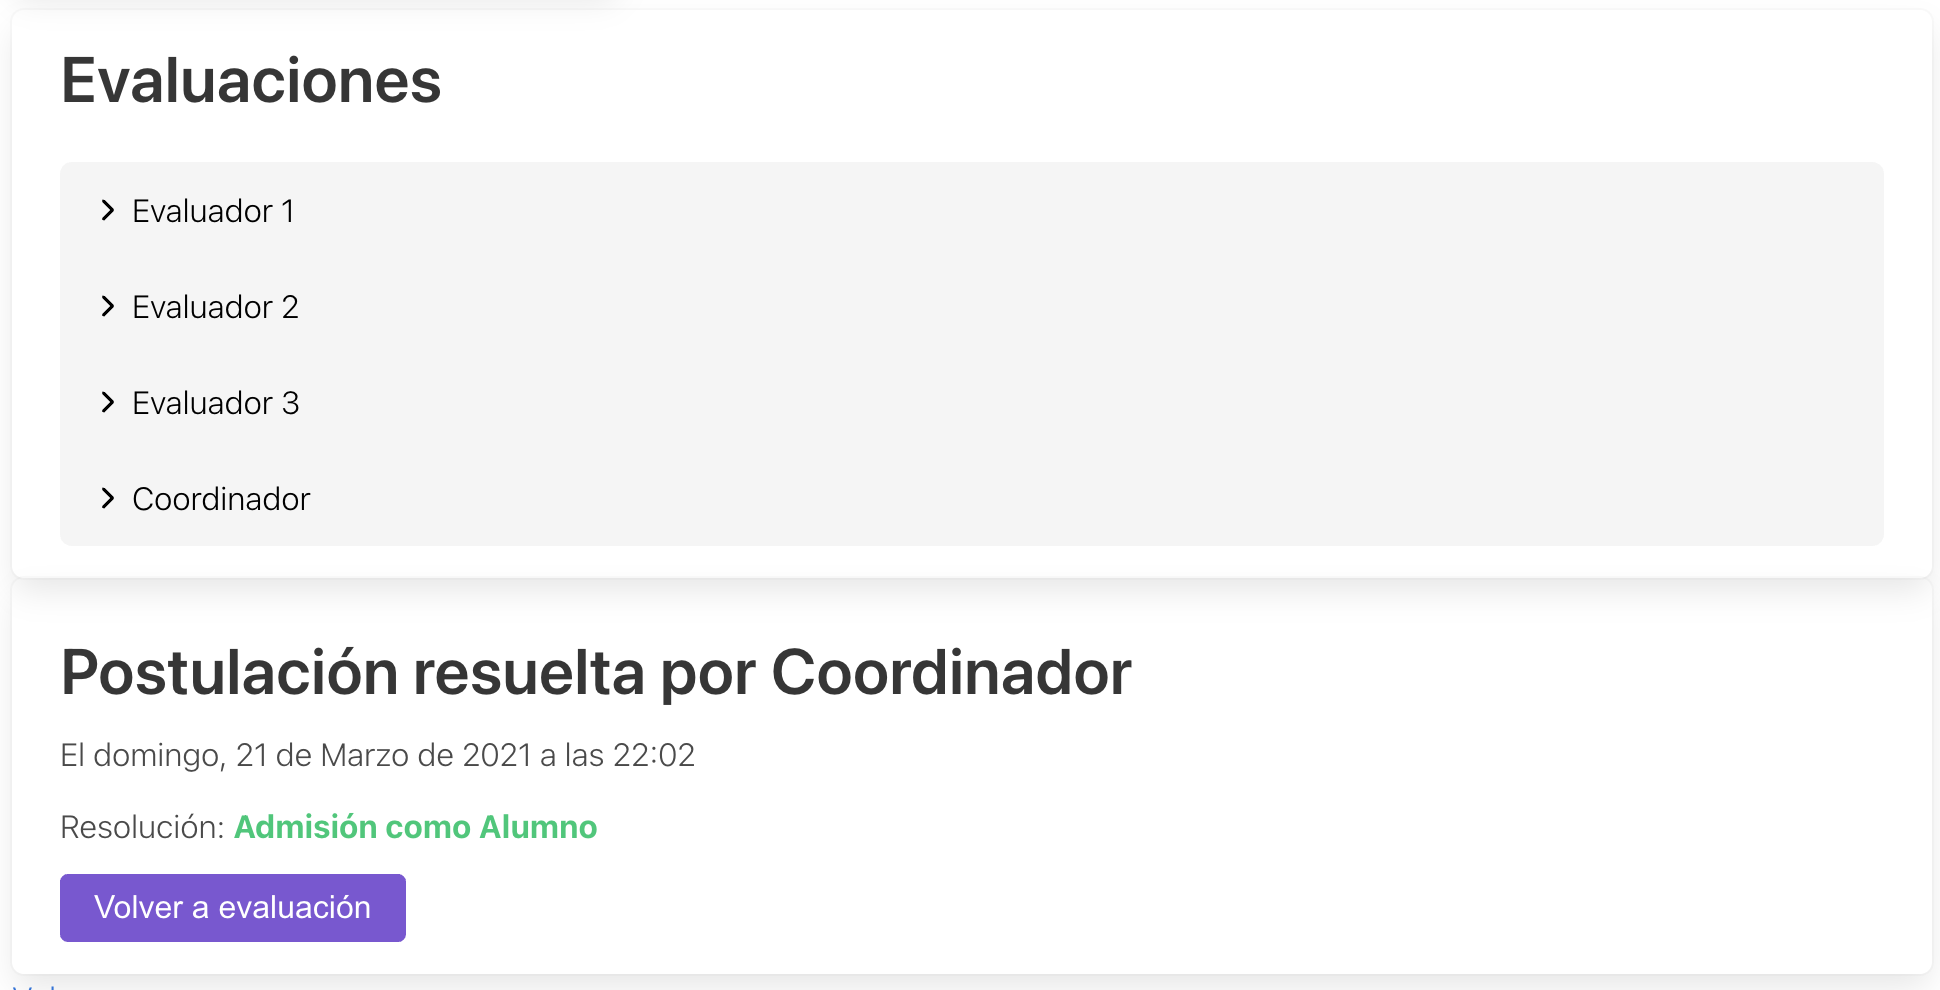
\includegraphics[scale=0.44]{imagenes/04-postulacion-resuelta.png}
    \end{center}
    \caption{Interfaz para el coordinador de una postulación resuelta}
    \label{fig:postulacion-resuelta}
\end{figure}
\chapter{Evaluación de la Solución}

A continuación se describe el proceso de evaluación realizado, los resultados
obtenidos y los aspectos de mejora de la aplicación.

\section{Proceso de Evaluación}

El proceso de evaluación del software se enfocó principalmente en determinar la
correctitud de operaciones realizadas por el sistema, y la adherencia de éste al
flujo de trabajo definido para cada uno de los participantes. Para las pruebas
el software se dejó disponible en el siguiente URL:
https://postulaciones.netlify.app/. Se ingresaron 17 postulaciones al sistema,
todas ellas con información ficticia, por razones de privacidad.

Además se definieron tres usuarios con perfil de \emph{asistente}, cuatro con perfil de
\emph{evaluador} (miembros del comité académico del programa) y un coordinador. La
evaluación fue hecha por los actuales coordinadores del Programa, quienes
asumieron temporalmente los distintos roles (perfiles de usuario) para llevar
adelante el proceso completo. Es importante destacar que estas personas han
participado en la evaluación de postulaciones durante al menos los últimos 10
años. 

Los distintos usuarios se autenticaron en la aplicación, y realizaron su labor
habitual utilizando el nuevo sistema. Particularmente, durante esta evaluación
los asistentes procesaron 12 de las 14 postulaciones disponibles. Los
evaluadores revisaron y emitieron un juicio sobre 11 de ellas, y el coordinador
decidió la aceptación o rechazo de sobre 6 postulaciones. Esto significa que se
realizó el flujo de trabajo completo para 6 postulaciones, involucrando a todos
los actores en el proceso. Además, se realizó una parte del flujo de trabajo
para otras 6 postulaciones.

El estado en que quedaron las postulaciones se muestra en la siguiente figura,
donde el estado “\emph{pendiente}” significa que el asistente aún no ha revisado
la postulación, y por lo tanto, no es posible evaluarla. El estado
“\emph{resuelta}”indica que los evaluadores emitieron su opinión, y el
coordinador resolvió en base a ellas. El estado “\emph{en evaluación por el
comité académico}” significa que la postulación está siendo evaluada, y que al
menos un miembro de dicho comité no ha emitido su opinión respecto a la
aceptación o rechazo de la misma. Finalmente, el estado “\emph{esperando
resolución}” significa que todos los miembros del comité académico han emitido
su opinión, y sólo resta que el coordinador decida y registre la decisión en
UCampus.

\begin{figure}[!ht]
    \begin{center}
        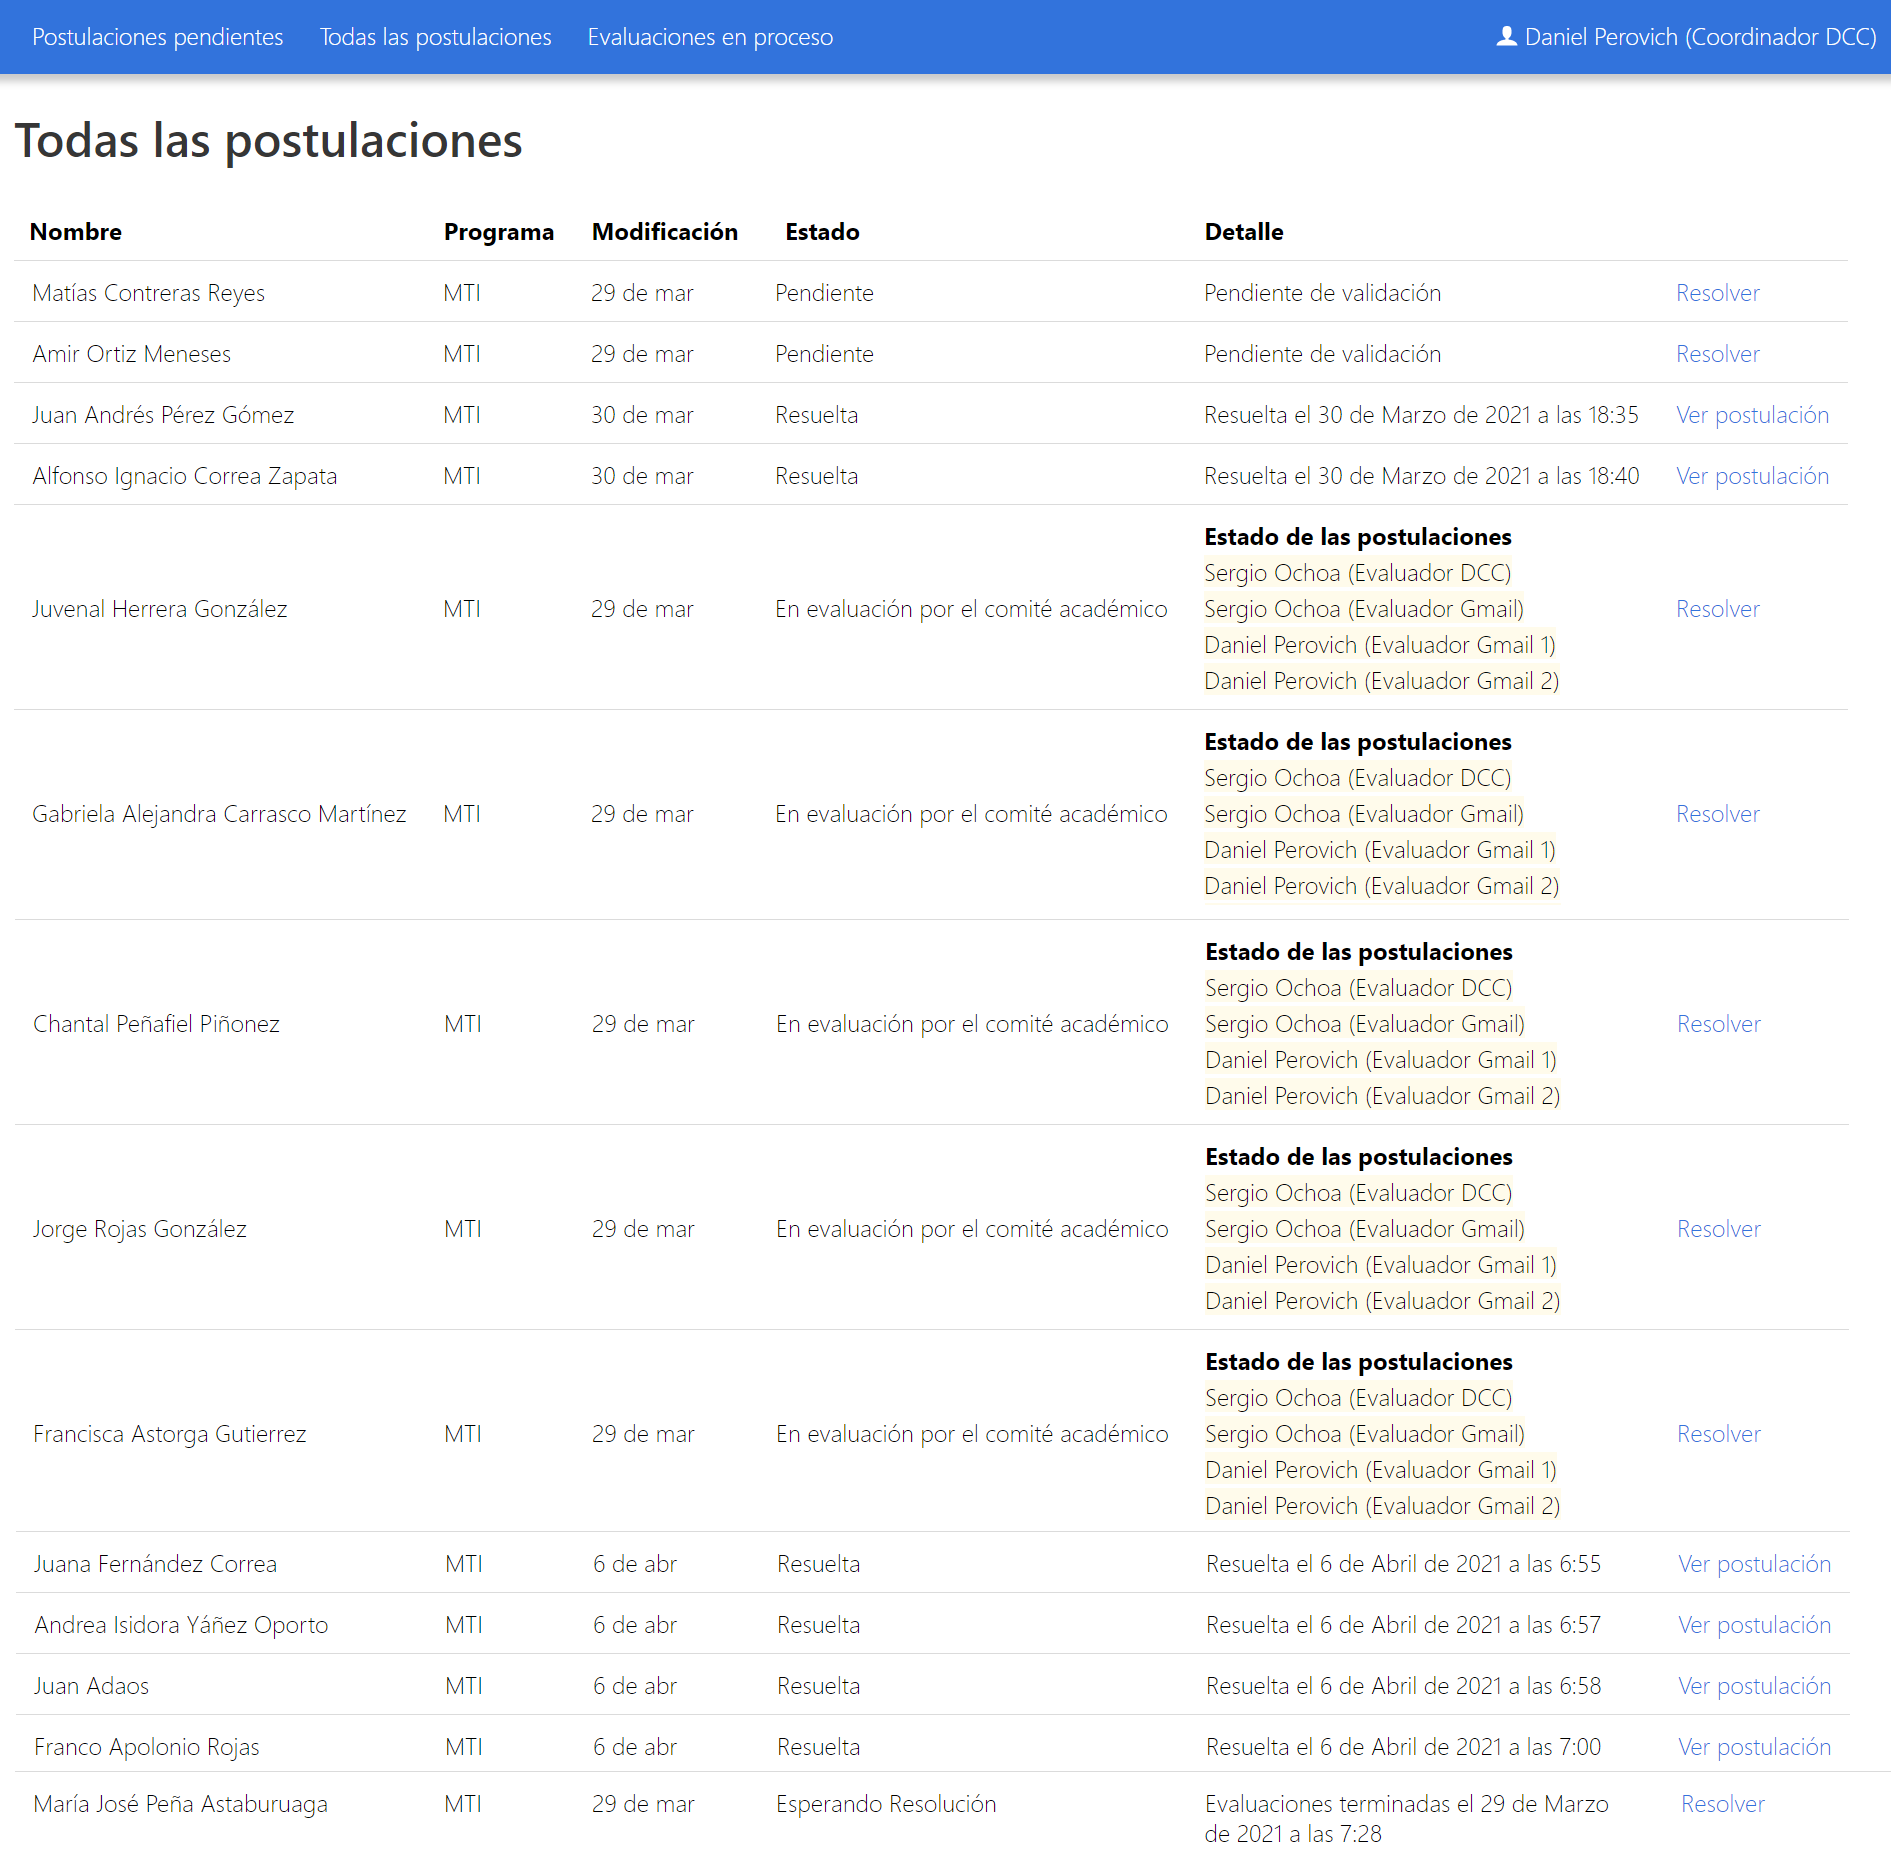
\includegraphics[scale=0.23]{imagenes/05-estado-final-evaluaciones.png}
    \end{center}
    \caption{Formulario de resolución de postulaciones}
    \label{fig:estado-final-evaluaciones}
\end{figure}

\section{Sobre los resultados obtenidos}

En primer lugar es importante destacar que la aplicación logró dar soporte al
workflow completo del proceso de evaluación, considerando los roles de los
participantes, y sin ningún error de lógica. Tampoco se detectó inestabilidad
del sistema, y su usabilidad fue calificada como “buena” por parte de los
usuarios. En ese sentido se puede afirmar que se alcanzaron los objetivos
definidos en esta memoria, y que la aplicación resultante está en condiciones de
probarse en marcha blanca con postulaciones reales.

Por otra parte, los usuarios hicieron varios comentarios orientados a mejorar
las interfaces del sistema, en pos de facilitar el trabajo de cada rol. También
observaron varios aspectos que restringen la información a la que pueden acceder
algunos roles, respecto de las postulaciones. A continuación se indican los más
importantes:

\begin{itemize}
    \item Que las tablas que muestran las postulaciones en los diferentes tracks
    permitan ordenar dichas postulaciones por columna, para así hacer más
    flexible y simple la identificación de postulaciones en diferentes estados,
    o bien identificar postulaciones en particular.
    \item Que los asistentes no puedan ver las evaluaciones hechas por los
    miembros del comité académico. Esto incluye la resolución propuesta y los
    comentarios realizados para cada uno de los ítems de evaluación. En resumen,
    los asistentes sólo podrán ver ver que la evaluación fue hecha por un
    evaluador un cierto día y hora.
    \item Un evaluador solo debe poder ver las postulaciones en las que
    participó como evaluador (independientemente de si realizó la evaluación, o
    se la cancelaron). Este tipo de usuario no debe poder ver las postulaciones
    en las que no participó. 
    \item Reemplazar las actuales tres opciones de menú, por las que se indican
    a continuación, solo por una cuestión de facilidad de comprensión y acceso a
    las postulaciones por parte de los diferentes usuarios:
    \begin{itemize}
        \item \emph{Postulaciones abiertas}. Mostrar todas las postulaciones que
        aún tienen tareas pendientes de ser realizadas, ordenadas de más
        antiguas a más nuevas por fecha de postulación.
        \item \emph{Postulaciones cerradas}. Mostrar todas las postulaciones que
        ya fueron resueltas (ya sea aceptadas o rechazadas), ordenadas de más
        nueva a más antiguas por fecha de postulación. usuario tiene asignadas
        para evaluar, ordenadas de más antiguas a más nuevas por fecha límite
        para hacer la evaluación.
        \item \emph{Evaluaciones pendientes}. Mostrar todas las postulaciones
        que el usuario tiene asignadas para evaluar, ordenadas de más antiguas a
        más nuevas por fecha límite para hacer la evaluación.
        \item \emph{Evaluaciones realizadas}. Mostrar todas las postulaciones que el
        usuario ya evaluó, ordenadas de más nueva a más antiguas por fecha en
        que fue realizada la evaluación.
    \end{itemize}
\end{itemize}

Es importante destacar que estos ajustes al sistema plantean reorganizar o
limitar el acceso a los servicios que ya están implementados. Por lo tanto, su
incorporación no significa un gran desafío para el proyecto, y son fácilmente
realizables.


\begin{conclusion}
	\lipsum[130-132]
	\begin{figure}[!h]
		\centering
		
\includegraphics[scale=.2]{imagenes/fcfm.pdf}
		\caption{Logo de la Facultad}
		\label{logofcfm}
	\end{figure}
	\lipsum[133-134]
	\begin{table}[!h]
		\centering
		\begin{tabular}{|c||c|}
			\hline
			Campo 1& Campo 2\\\hline
			Valor 1& Valor2\\\hline
		\end{tabular}
		\caption{Tabla 1}
		\label{tabla:1}
	\end{table}
	\lipsum[135]
\end{conclusion}


\nocite{*}
\bibliographystyle{plain}
\bibliography{bibliografia}
\end{document}
